\section*{Общая характеристика работы}

\newcommand{\actuality}{\underline{\textbf{\actualityTXT}}}
\newcommand{\progress}{\underline{\textbf{\progressTXT}}}
\newcommand{\aim}{\underline{{\textbf\aimTXT}}}
\newcommand{\tasks}{\underline{\textbf{\tasksTXT}}}
\newcommand{\novelty}{\underline{\textbf{\noveltyTXT}}}
\newcommand{\appropriation}{\underline{\textbf{\appropriationTXT}}}
\newcommand{\influence}{\underline{\textbf{\influenceTXT}}}
\newcommand{\methods}{\underline{\textbf{\methodsTXT}}}
\newcommand{\defpositions}{\underline{\textbf{\defpositionsTXT}}}
\newcommand{\reliability}{\underline{\textbf{\reliabilityTXT}}}
\newcommand{\probation}{\underline{\textbf{\probationTXT}}}
\newcommand{\contribution}{\underline{\textbf{\contributionTXT}}}
\newcommand{\publications}{\underline{\textbf{\publicationsTXT}}}


{\actuality} 
Актуальность темы обоснована стремительным развитием нейросетевых моделей. В последнее время нейросетевые модели на основе трансформеров, типа BERT, стали чаще применяться в различных областях, в том числе в диалоговых системах. Это связано с тем, что они показывают более высокие результаты, чем иные методы машинного обучения. В то же самое время, такие модели требуют вычислительных ресурсов, которые могут быть дорогостоящими. В связи с этим развитие получает идея многозадачного обучения - использование одной и той же модели для решения нескольких задач машинного обучения. Тем не менее, перенос данных в многозадачных нейросетевых моделях между задачами и языками, особенно для задач, применимых в диалоговых системах, всё еще не изучены до конца. Наборов данных в открытом доступе для задач диалоговых систем, таких, как тематическая классификация, также недостаточно.


{\aim} данной работы является определение закономерностей, влияющих на перенос знаний между языками и задачами в многозадачных нейросетевых моделях на различных архитектурах, а также на особенности прикладного применения этих моделей в диалоговой платформе.

Для достижения поставленной цели необходимо было решить следующие {\tasks}:

\begin{enumerate}
  \item {Создать и выложить в открытый доступ диалоговую платформу, на которой в дальнейшем могло бы изучаться прикладное применение многозадачных нейросетевых моделей. Проверить качество этой диалоговой платформы оценками пользователей.}
  \item {Проверить применимость технологий, использованных в диалоговой платформе DREAM, в иных прикладных задачах.}
  \item {Провести эксперименты для сравнения различных схем псевдоразметки данных для многозадачных нейросетевых моделей с одним линейным слоем.}
  \item {Провести эксперименты для сравнения различных вариантов выбора архитектуры многозадачных нейросетевых моделей, а также выбора сэмплирования для определенных типов таких моделей.}
  \item {Провести эксперименты для анализа закономерностей переноса знаний в трансформер-агностичных многозадачных нейросетевых моделях между различными диалоговыми задачами. В частности, провести оценку зависимости этого переноса от размера обучающей выборки.}
  \item {Провести эксперименты для анализа закономерностей переноса знаний в многоязычных трансформер-агностичных многозадачных нейросетевых моделях между различными языками - с английского языка на русский. В частности, провести оценку зависимости этого переноса от размера обучающей выборки. Рассмотреть также применимость этих выводов для однозадачных моделей.}
  \item {Проверить пригодность русскоязычного открытого набора тематических данных для решения задачи русскоязычной тематической классификации и фундаментальных задач исследования переноса знаний на разговорных данных.}
  \item {Проверить зависимость межъязыкового переноса знаний на разговорных данных в многоязычных нейросетевых моделях от размера предобучающей выборки и генеалогической близости языков.}
  \item {Интегрировать рассмотренные в диссертации многозадачные нейросетевые архитектуры в диалоговую платформу, оценить применимость данных архитектур и провести их сравнительный анализ на основе опыта практического применения. На основании этого анализа произвести интеграцию также в open-source библиотеку.}
  \newline
  \newline
\end{enumerate}


{\novelty}
\begin{enumerate}
  \item {Создана и выложена в открытый доступ диалоговая платформа DREAM, на которй в дальнейшем может изучаться прикладное применение многозадачных нейросетевых моделей. Качество этой диалоговой платформы было проверено оценками пользователей в рамках конкурса "Alexa Prize Socialbot Grand Challenge", по результатам которых платформа DREAM вышла в полуфинал этого конкурса.}
  \item {Проверена применимость технологий, использованных в диалоговой платформе DREAM, на прикладной задаче по созданию сервиса для работы с текстами texter-ocr-cv-microservice.}
  \item {Проведены эксперименты для сравнения различных схем псевдоразметки данных для многозадачных нейросетевых моделей с одним линейным слоем на примере задач из набора данных GLUE.}
  \item {Проведены эксперименты для сравнения различных вариантов выбора архитектуры многозадачных трансформер-агностичных нейросетевых моделей, сравнения их с аналогичными однозадачными моделями для разных тел, а также выбора сэмплирования для определенных типов таких моделей.}
  \item {Проведены эксперименты для анализа закономерностей переноса знаний в трансформер-агностичных многозадачных нейросетевых моделях между различными диалоговыми задачами. В частности, была произведена оценка зависимости этого переноса от размера обучающей выборки.}
  \item {Проведены эксперименты для анализа закономерностей переноса знаний в многоязычных трансформер-агностичных многозадачных нейросетевых моделях между различными языками - с английского языка на русский. В частности, была проведена оценка зависимости этого переноса от размера обучающей выборки. Была рассмотрена также применимость этих выводов для однозадачных моделей.}
  \item {Проверена пригодность хотя бы 1 русскоязычного открытого набора тематических данных \texttt{YAQTopics} для решения задачи русскоязычной тематической классификации и фундаментальных задач исследования переноса знаний.}
  \item {Проверена зависимость межъязыкового переноса знаний на разговорных данных в многоязычных нейросетевых моделях от размера предобучающей выборки и генеалогической близости языков.}
  \item {Рассмотренные в диссертации многозадачные нейросетевые архитектуры были интегрированы в диалоговую платформу DREAM, была оценена применимость и был проведен их сравнительный анализ на основе опыта применения. На основании этого анализа была произведена также интеграция в open-source библиотеку DeepPavlov} 
\end{enumerate}

{\appropriation}
Пункты 3,4, 5, 6, 7 и 8 Научной новизны соответствуют Пункту 8 "Комплексные исследования научных и технических проблем с применением современной технологии математического моделирования и
вычислительного эксперимента." специальности 1.2.2 «Математическое моделирование, численные методы и комплексы программ». специальности 1.2.2 «Математическое моделирование, численные методы и комплексы программ», так как предложенный набор данных может использовать для валидации различных моделей машинного обучения. Пункты 1,2 и 9 Научной новизны соответствует пункту 6 "Разработка систем компьютерного и имитационного моделирования, алгоритмов и методов имитационного моделирования на основе анализа математических моделей" специальности 1.2.2 «Математическое моделирование, численные методы и комплексы программ».

{\defpositions}
\begin{enumerate}
  \item {Диалоговая платформа \texttt{DREAM} пригодна для изучения прикладного применения многозадачных нейросетевых моделей. Оценки пользователей в рамках международного конкурса "Alexa Prize Socialbot Grand Challenge", обеспечившие двукратный выход в полуфинал этой платформы, показывают высокое качество диалоговой платформы на момент её создания.}
  \item {На примере прикладной задачи по созданию сервиса для работы с текстами texter-ocr-cv-microservice показана применимость технологий, использованных в диалоговой платформе DREAM, за пределами этой диалоговой платформы.}
  \item {Псевдоразметка данных при помощи однозадачных моделей улучшает метрики многозадачных моделей. При этом объединение классов оправдывает себя только для задач, достаточно сильно похожих друг на друга.}
  \item {Было показано на различных наборах данных, что многозадачные трансформер-агностичные нейросетевые модели показывают себя не хуже ряда других, более сложных архитектур, а предложенный метод сэмплирования - не хуже ряда других методов сэмплирования. При этом многозадачные трансформер-агностичные модели по данным проведенным экспериментах дают среднюю просадку не более 1 процента по сравнению с однозадачными моделями. А если какие-то задачи достаточно похожи друг на друга, как например, в бенчмарке GLUE, многозадачные модели за счет таких задач в среднем даже превосходят однозадачные модели.}
  \item {Было показано, что для достаточно малых данных многозадачные трансформер-агностичных модели начинают превосходить по своей средней точности однозадачные, в особенности - за счет задач с наименьшим объемом данных.}
  \item {Было показано, что если в основе многозадачной трансформер-агностичной модели лежит многоязычный BERT, то добавление английских данных к русским при соответствующей номенклатуре классов позволяет улучшить метрики на 1-5\%. Чем меньше изначально русскоязычных данных, тем улучшение сильнее. Этот же вывод справедлив и для однозадачных моделей.}
  \item {Русскоязычный открытый набор тематических данных \texttt{YAQTopics} пригоден для решения задачи русскоязычной тематической классификации и фундаментальных задач исследования переноса знаний.}
  \item {Для многоязычных нейросетевых моделей качество переноса знаний на разные языки на тематических данных сильно коррелирует с размером предобучающей выборки для каждого языка, но при этом не коррелирует с генеалогической близостью этого языка к русскому.}
  \item {Рассмотренные многозадачные нейросетевые архитектуры пригодны для практического применения в диалоговых платформах и в рамках open-source библиотек. При этом предложенные автором трансформер-агностичные нейросетевые модели выигрывают у моделей типа PAL-BERT за счет трансформер-агностичности, а у моделей с одним линейным слоем - за счёт большей гибкости, отсутствия необходимости в псевдоразметке и как следствие - меньшей склонности к переобучению.}
\end{enumerate}


\iffalse
Направления исследований 1.2.2:
1. Разработка новых математических методов моделирования объектов и
явлений (физико-математические науки).
2. Разработка, обоснование и тестирование эффективных вычислительных
методов с применением современных компьютерных технологий.
3. Реализация эффективных численных методов и алгоритмов в виде
комплексов проблемно-ориентированных программ для проведения
вычислительного эксперимента.
4. Разработка новых математических методов и алгоритмов интерпретации
натурного эксперимента на основе его математической модели.
5. Разработка новых математических методов и алгоритмов валидации
математических моделей объектов на основе данных натурного эксперимента
или на основе анализа математических моделей.
6. Разработка систем компьютерного и имитационного моделирования,
алгоритмов и методов имитационного моделирования на основе анализа
математических моделей (технические науки).
7. Качественные или аналитические методы исследования математических
моделей (технические науки).
8. Комплексные исследования научных и технических проблем с
применением современной технологии математического моделирования и
вычислительного эксперимента.
9. Постановка и проведение численных экспериментов, статистический
анализ их результатов, в том числе с применением современных
компьютерных технологий (технические науки).
\fi


{\influence}
Практическая значимость заключается в следующем. Впервые в России была разработана диалоговая платформа мирового уровня, вышедшая в полуфинал престижных мировых конкурсов Alexa Prize 3 и Alexa Prize 4 (в конкурсах было 10 и 9 участников соответственно, из более чем 300 кандидатов). Эта диалоговая платформы имеет полностью открытый код, что дает возможность легкого переиспользования любой части проделанной над ней работы. 

В этой платформе, в числе всего прочего, применялись многозадачные нейросетевые модели, описанные автором в данном работе - многозадачная нейросетевая модель с одним линейным слоем, многозадачная нейросетевая модель на основе архитектуры PAL-BERT и многозадачная трансформер-агностичная нейросетевая модель. Был проведен ряд других прикладных работ для улучшения данной платформы, включающий в себя разработку сценарных навыков.

Помимо этого, программный код для реализации многозадачной трансформер-агностичной нейросетевой модели встроен в библиотеку DeepPavlov, имеющую более 500 000 скачиваний на март 2023 года.
Алгоритмы, использованные в данной работе, применены также в программе для ЭВМ [А6], на которую получено свидетельство о государственной регистрации.


{\methods}
В данной работе были
применены:
\begin{enumerate}
\item Метод численного эксперимента для исследования задач обработки естественного языка;
\item Основы теории вероятностей;
\item Методы машинного обучения и теории глубокого обучения;
\item Методы разработки на языках Python, Bash.
\end{enumerate}




{\reliability} полученных результатов обеспечивается экспериментами на наборах диалоговых данных и наборе данных GLUE, описанными в~\cite{pseudolabel}(индексируется в Scopus), ~\cite{Болотин_Карпов_Рашков_Шкурак_2019}, ~\cite{rumtl},~\cite{enmtl},~\cite{rutopics},~\cite{dp_2023}, применением в соревнованиях "Alexa Prize Challenge 3" и "Alexa Prize Challenge 4", описанным в ~\cite{dream1}, ~\cite{dream2}, ~\cite{dream1_trudy}(входит в список ВАК), а также использованием результатов работы в диалоговой платформе \texttt{DREAM} и библиотеке DeepPavlov. Результаты находятся в соответствии с результатами, полученными другими авторами.


{\probation}
Апробация работы. Результаты работы были представлены автором на конференции Диалог-2021~\cite{pseudolabel}, и опубликованы в журналах Proceedings of En\&T 2018~\cite{Болотин_Карпов_Рашков_Шкурак_2019}, Computational Linguistics and Information Technologies~\cite{pseudolabel,rumtl},Proceedings of Alexa Prize 3~\cite{dream1},Proceedings of Alexa Prize 4~\cite{dream2}, Труды МФТИ~\cite{dream1_trudy}, Proceedings of AINL 2023~\cite{rutopics}, Proceedings of InterSpeech 2023~\cite{enmtl}, Proceedings of ACL Systems Workshop~\cite{dp_topics}. Помимо этого, разработки, описанные в данной диссертации, были внедрены в находящуюся в открытом доступе диалоговую платформу \texttt{DREAM}, активно используемую в конкурсах Alexa Prize 3, Alexa Prize 4 и после них. Также на разработки, основанные на результатах работы, было получено свидетельство о регистрации ПО~\cite{Дуплякин_Дмитрий_Ондар_Ушаков_2021}.


{\contribution} В работе~\cite{Болотин_Карпов_Рашков_Шкурак_2019} автор отвечал за ряд важных компонент диалоговой системы, включающих в себя парафразер. Исследование, разработка и сравнительный анализ методов псевдоразметки данных, описанных в работе~\cite{pseudolabel}, были выполнены автором самостоятельно. В работах~\cite{dream1,dream1_trudy,dream2} автор отвечал за ряд важных компонент диалоговой системы - навыки обсуждения книг, эмоций, коронавируса, классификаторы эмоций,интентов,момента остановки диалога, TF-IDF Retrieval, Grounding Skill, Gossip Skill, генеративный навык и многозадачную нейросетевую модель. Технические решения для работы с естественным языком, использованные в \cite{dream1,dream1_trudy,dream2}, использовались также в~\cite{Дуплякин_Дмитрий_Ондар_Ушаков_2021}. В работах~\cite{rumtl,enmtl,rutopics} все исследования также были выполнены автором самостоятельно. В работе~\cite{dp_2023} автор отвечал за эксперименты с многозадачными трансформер-агностичными моделями для библиотеки DeepPavlov и их описание.

\ifnumequal{\value{bibliosel}}{0}
{%%% Встроенная реализация с загрузкой файла через движок bibtex8. (При желании, внутри можно использовать обычные ссылки, наподобие `\cite{vakbib1,vakbib2}`).
    {\publications} 

}%
{%%% Реализация пакетом biblatex через движок biber
    \begin{refsection}[bl-author]
        % Это refsection=1.
        % Процитированные здесь работы:
        %  * подсчитываются, для автоматического составления фразы "Основные результаты ..."
        %  * попадают в авторскую библиографию, при usefootcite==0 и стиле `\insertbiblioauthor` или `\insertbiblioauthorgrouped`
        %  * нумеруются там в зависимости от порядка команд `\printbibliography` в этом разделе.
        %  * при использовании `\insertbiblioauthorgrouped`, порядок команд `\printbibliography` в нём должен быть тем же (см. biblio/biblatex.tex)
        %
        % Невидимый библиографический список для подсчёта количества публикаций:
        \printbibliography[heading=nobibheading, section=1, env=countauthorvak,          keyword=biblioauthorvak]%
        \printbibliography[heading=nobibheading, section=1, env=countauthorwos,          keyword=biblioauthorwos]%
        \printbibliography[heading=nobibheading, section=1, env=countauthorscopus,       keyword=biblioauthorscopus]%
        \printbibliography[heading=nobibheading, section=1, env=countauthorconf,         keyword=biblioauthorconf]%
        \printbibliography[heading=nobibheading, section=1, env=countauthorother,        keyword=biblioauthorother]%
        \printbibliography[heading=nobibheading, section=1, env=countauthor,             keyword=biblioauthor]%
        \printbibliography[heading=nobibheading, section=1, env=countauthorvakscopuswos, filter=vakscopuswos]%
        \printbibliography[heading=nobibheading, section=1, env=countauthorscopuswos,    filter=scopuswos]%
        %
        \nocite{*}%
        %
        {\publications} Основные результаты по теме диссертации изложены в~\arabic{citeauthor}~печатных изданиях,
        \arabic{citeauthorvak} из которых изданы в журналах, рекомендованных ВАК\sloppy%
        \ifnum \value{citeauthorscopuswos}>0%
            , \arabic{citeauthorscopuswos} "--- в~периодических научных журналах, индексируемых Web of~Science и Scopus\sloppy%
        \fi%
        \ifnum \value{citeauthorconf}>0%
            , \arabic{citeauthorconf} "--- в~тезисах докладов.
        \else%
            .
        \fi
    \end{refsection}%
    \begin{refsection}[bl-author]
        % Это refsection=2.
        % Процитированные здесь работы:
        %  * попадают в авторскую библиографию, при usefootcite==0 и стиле `\insertbiblioauthorimportant`.
        %  * ни на что не влияют в противном случае
        \nocite{Болотин_Карпов_Рашков_Шкурак_2019}%vak
        \nocite{dream1}%vak
        \nocite{dream2}%vak
        \nocite{pseudolabel}
        \nocite{dream1_trudy}%vak
        \nocite{Дуплякин_Дмитрий_Ондар_Ушаков_2021}%vak
        \nocite{rumtl}
        \nocite{rutopics}
        \nocite{enmtl}
        \nocite{dp_2023}
    \end{refsection}%
        %
        % Всё, что вне этих двух refsection, это refsection=0,
        %  * для диссертации - это нормальные ссылки, попадающие в обычную библиографию
        %  * для автореферата:
        %     * при usefootcite==0, ссылка корректно сработает только для источника из `external.bib`. Для своих работ --- напечатает "[0]" (и даже Warning не вылезет).
        %     * при usefootcite==1, ссылка сработает нормально. В авторской библиографии будут только процитированные в refsection=0 работы.
        %
        % Невидимый библиографический список для подсчёта количества внешних публикаций
        % Используется, чтобы убрать приставку "А" у работ автора, если в автореферате нет
        % цитирований внешних источников.
        % Замедляет компиляцию
    \ifsynopsis
    \ifnumequal{\value{draft}}{0}{
      \printbibliography[heading=nobibheading, section=0, env=countexternal,          keyword=biblioexternal]%
    }{}
    \fi
}
\iffalse
При использовании пакета \verb!biblatex! будут подсчитаны все работы, добавленные
в файл \verb!biblio/author.bib!. Для правильного подсчёта работ в~различных
системах цитирования требуется использовать поля:
\begin{itemize}
        \item \texttt{authorvak} если публикация индексирована ВАК,
        \item \texttt{authorscopus} если публикация индексирована Scopus,
        \item \texttt{authorwos} если публикация индексирована Web of Science,
        \item \texttt{authorconf} для докладов конференций,
        \item \texttt{authorother} для других публикаций.
\end{itemize}
Для подсчёта используются счётчики:
\begin{itemize}
        \item \texttt{citeauthorvak} для работ, индексируемых ВАК,
        \item \texttt{citeauthorscopus} для работ, индексируемых Scopus,
        \item \texttt{citeauthorwos} для работ, индексируемых Web of Science,
        \item \texttt{citeauthorvakscopuswos} для работ, индексируемых одной из трёх баз,
        \item \texttt{citeauthorscopuswos} для работ, индексируемых Scopus или Web of~Science,
        \item \texttt{citeauthorconf} для докладов на конференциях,
        \item \texttt{citeauthorother} для остальных работ,
        \item \texttt{citeauthor} для суммарного количества работ.
\end{itemize}
% Счётчик \texttt{citeexternal} используется для подсчёта процитированных публикаций.

Для добавления в список публикаций автора работ, которые не были процитированы в
автореферате требуется их~перечислить с использованием команды \verb!\nocite! в
\verb!Synopsis/content.tex!.
\fi
 % Характеристика работы по структуре во введении и в автореферате не отличается (ГОСТ Р 7.0.11, пункты 5.3.1 и 9.2.1), потому её загружаем из одного и того же внешнего файла, предварительно задав форму выделения некоторым параметрам

%Диссертационная работа была выполнена при поддержке грантов \dots

%\underline{\textbf{Объем и структура работы.}} Диссертация состоит из~введения,
%четырех глав, заключения и~приложения. Полный объем диссертации
%\textbf{ХХХ}~страниц текста с~\textbf{ХХ}~рисунками и~5~таблицами. Список
%литературы содержит \textbf{ХХX}~наименование.
\section*{Содержание работы}
Во \underline{\textbf{введении}} обосновывается актуальность
исследований, проводимых в~рамках данной диссертационной работы,
приводится обзор научной литературы по изучаемой проблеме,
формулируется цель, ставятся задачи работы, излагается научная новизна
и практическая значимость представляемой работы. 

\underline{\textbf{Первая глава}} является обзорной. В этой главе дается определение нейросетевых методов машинного обучения для задач обработки естественного языка. 
Дается представление о различных базовых понятиях, таких, как метод обратного распространения ошибки, полносвязная архитектура и токенизация. 

Нейросетевые методы машинного обучения -- это методы, основанные на использовании искусственных нейронных сетей. В данной работе рассматривается класс искусственных нейронных сетей, представляющих собой совокупность слоев с функциями активации, таких, что подаваемые на вход данные проходят через различные слои по очереди, где каждый слой представляет собой многомерную функцию многих переменных. Итоговый выход нейронной сети подается в функцию потерь, после чего функция потерь оптимизируется методом обратного распространения ошибки. 

Метод обратного распространения ошибки -- один из методов «обучения с учителем», то есть подход, при котором модель учится решать задачу, чтобы соответствовать набору примеров входных/выходных данных. Для определения того, насколько ответ, данный нейронной сетью, соответствует требуемому, вводится функция потерь. Далее выполняется поиск точки минимума функции потерь в пространстве параметров искусственной нейронной сети для данного набора примеров входных данных. 

Все самые главные достижения в области нейронных сетей в 21 веке были связаны именно с применением нейросетевых подходов. 

Одним из классических видов нейронных сетей являются полносвязные нейронные сети -- сети, состоящие из полносвязных слоев. Будем называть полносвязным слоем с M нейронами взвешенную сумму значений входного вектора x размерности N, к каждому элементу которой затем применяется функция активации $\sigma(y)$:

\begin{equation}
\begin{split} 
\color{black}z=\sigma(y)\\
\color{black}y=W_{0}+W_{1}X
\end{split}
\label{nn:0}
\end{equation}
где $W_{1}$ -- матрица весов (weights) полносвязного слоя размерности $N*M$, $W_{0}$ -- матрица биасов (bias) полносвязного слоя размерности M, $\sigma$ -- некая нелинейная функция активации.

Для регуляризации в таких слоях (как и в других, более сложных) применяется также дропаут -- метод, при котором некий процент элементов выходного вектора (как правило, 10-20\%) приравнивается к нулю. Такая техника мешает «переобучению» нейронной сети, улучшая тем самым ее обобщающую способность.

Токенизация текста -- это его разбиение на элементарные единицы(токены) перед предобработкой. Один токен соответствует одному слову и/или одной его части в зависимости от метода токенизации. Для нижеописанного метода Word2Vec токеном является 1 слово, для нижеописанной архитектуры BERT -- слово либо слог.

Помимо этого, в первой главе разбираются нейросетевые архитектуры, которые использовались в данной диссертационной работе. В частности, разбирается архитектура Трансформер и нейросетевая модель {BERT}, основанная на данной архитектуре.

Последний раздел главы посвящен многозадачным нейросетевым моделям. В нём даётся определение многозадачного обучения и приводится классификация многозадачных нейросетевых архитектур.

Многозадачное обучение -- это метод разделения параметров между моделями, обучающимися выполнять несколько задач. Все имеющиеся многозадачные нейросетевые архитектуры можно разделить на четыре типа:
\begin{itemize}
\item Параллельные архитектуры. Для данного типа архитектур одни и те же «общие» слои используются для примеров из каждой задачи, при этом выход «общих» слоев обрабатывается независимо своим специфическим слоем для каждой задачи. 
\item Иерархические архитектуры. Для данного типа архитектур задачи обрабатываются зависимо друг от друга: так, результат классификации примера для одной из задач может использоваться при решении другой из задач как дополнительный входной параметр.
\item Модульные архитектуры. Нейронная сеть в данных архитектурах делится на общие модули и задаче-специфичные модули, где общие модули имеют одни и те же веса для всех задач, а задаче-специфичные модули -- свои веса для каждой из задач.
\item Генеративно-состязательные архитектуры. Для данного типа архитектур генератор и дискриминатор обучаются совместно таким образом, что дискриминатор пытается предсказать, из какой задачи пример, по его выдаваемому генератором представлению. А генератор, соответственно, пытается сгенерировать такое представление, чтобы дискриминатор мог предсказать задачу как можно хуже. 
\end{itemize}
В завершении первого раздела приводится подробный обзор двух архитектур, на которых основывались последующие разделы данной диссертационной работы. А именно, модель {MT-DNN}, имеющая параллельную архитектуру, и модель {PAL-BERT}, имеющая модульную архитектуру. 

В связи с тем, что в многозадачных нейросетевых архитектурах один и тот же её элемент в том или ином виде может использоваться для решения нескольких задач, возможна такая ситуация, когда знания, полученные при обучении модели решать одну из задач, помогают при решении и другой задачи. Т.е модель, которая обучалась решать задачу A и задачу B, может показать себя на задаче B лучше, чем если бы она обучалась решать только задачу A. Данный эффект называется переносом знаний, и его изучение является частью диссертационной работы.

Главный {вывод} из первой главы заключается в том, что модели, основанные на описанных в данной главе нейросетевых архитектурах, пригодны для изучения многозадачного переноса знаний.

\underline{\textbf{Вторая глава}} посвящена многозадачным нейросетевым моделям с одним линейным слоем -- простейшему типу многозадачных моделей. Такие модели имеют архитектуру, аналогичную модели типа BERT для многометочной классификации (один линейный слой поверх модели, каждый нейрон в финальном слое может принимать значения от 0 до 1), при этом в финальном линейном слое разные нейроны отвечают за разные задачи.

В данной главе проводились эксперименты на следующих задачах из набора данных GLUE:
\begin{enumerate}
    \item QQP -- задача классификации пар предложений из сайта Quora.com на 2 класса -- и не дубликат.
    \item MNLI -- задача классификации пар предложений из различных тем на три класса -- логическое следование, логическое противоречие и нейтральный(ни следование, ни противоречие). Валидационный и тестовый наборы данных в MNLI существуют в 2 вариантах -- из тех же тем, что и тренировочный(MNLI-m) и из остальных тем (MNLI-mm).
    \item SST-2 -- задача классификации предложений на два класса -- положительная тональность и отрицательная тональность.
    \item RTE -- задача классификации пар предложений на два класса -- логическое следствие и нет логического следствия.
\end{enumerate}

Для этих задач сравниваются различные способы псевдоразметки данных при обучении многозадачной модели с одним линейным слоем,:
\begin{enumerate}
\item Базовый способ -- стандартное обучение однозадачных моделей.
\item Независимые метки -- метки для каждой задачи считаются независимыми (т.е всего девять классов), каждый пример имеет метку 1 для того класса своей задачи, к которому он принадлежит и 0 для всех остальных классов всех остальных задач. 
\item Независимые метки, замороженная голова -- аналогично режиму Независимые метки, но линейный слой заморожен и обучается только тело модели.
\item Мягкие независимые метки -- аналогично предыдущему подходу, но вероятности всех остальных классов каждой из остальных задач считаются равными друг другу так, чтобы их сумма равнялась 1. 
\item Мягкие независимые метки, замороженная голова -- аналогично режиму Мягкие независимые метки, но линейный слой заморожен и обучается только тело модели.
\item Дополненные независимые метки -- аналогичен режиму Мягкие независимые метки, но вероятности для всех классов каждой из остальных задач получаются при помощи предсказаний однозадачной модели, обученной исключительно на этой задаче.
\item Мягкое вероятностное предположение -- объединение классов с сокращением их числа до пяти: положительный, отрицательный, логическое следствие, логическое противоречие, нейтральный. В остальном та же логика, что и для режима Мягкие независимые метки.
\item Мягкие предсказанные метки -- аналогичен предыдущему, но все недостающие вероятности для каждой из задач не считаются равновероятными, а определяются дополнительной разметкой от модели для каждой задачи. 
\item Жесткие предсказанные метки -- аналогичен предыдущему, но для меток, полученных из предсказаний оригинальной модели, максимальная вероятность для каждой задачи округляется до 1, а все остальные вероятности до 0.
\end{enumerate}

\begin{table}[htbp]
\centering
\caption {Лучшая точность на тестовых данных (при лучшей скорости обучения из выбираемых, среднее по 3 запускам)}
\label{tab:ps2}% label всегда желательно идти после caption
\resizebox{\textwidth}{!}
{%
\begin{tabular}{|c||c|c|c|c|c|c|}
\hline
\multirow{2}{*}{Эксперимент} & \multicolumn{6}{c|}{Задача}  \\
\cline{2-7}
 & Среднее& RTE& QQP& MNLI-m &MNLI-mm& SST-2\\
\hline
Базовый (оригинальная статья) & 78.8 & 66.4  & 71.2 & 84.6 & 83.4 & 93.5 \\
\hline
Базовый (воспроизведённый) & 77.6 & 62.7 & 71.0 & 83.1 & 82.7 & 93.5 \\
\hline
Независимые метки &79.0 & 71.5 & 70.9 & 82.7 & 81.7 & 91.3 \\
\hline
Мягкие независимые метки  &78.9 & 69.3 & 71.3 & 82.8 & 82.1 & 92.6 \\
\hline
Дополненные независимые метки &77.6 & 64.2&\textbf{ 71.8} & 81.2 & 80.7 & \textbf{93.2} \\
\hline
Мягкое вероятностное предположение  &\textbf{79.7} & \textbf{72.7} & 70.7 &\textbf{ 83.4} &\textbf{82.3} & 92.5 \\
\hline
Мягкие предсказанные метки  & 78.8 & 70.3 & 70.7 & 81.7 & 81.7 & 92.5 \\
\hline
Жесткие предсказанные метки & 79.1 & 71.3 &71.1 & 81.7 & 81.4 & 92.6 \\
\hline
\begin{tabular}[c]{@{}l@{}}Независимые метки,\\замороженная голова\end{tabular}   & 78.2 & 66.9& \textbf{71.8} & 82.6 & 81.8 & 91.9 \\
\hline
\begin{tabular}[c]{@{}l@{}}Мягкие независимые метки,\\замороженная голова\end{tabular}  &79.1 & 70.0 & 71.5 & 83.0 &\textbf{ 82.3} & 92.4 \\
\hline
\end{tabular}
}
\end{table}


На задачах, сильнее всего похожих друг на друга (MNLI и RTE) лучше всего показывают себя способы, подразумевающие объединение меток, что говорит о том, что в определенных случаях оно может быть оправдано. 

С другой стороны, объединение меток не даёт улучшений для более разнородных задач, таких, как QQP и SST, что показывает ограничения этого метода. Лучше всего для таких задач показывает себя метод Дополненные независимые метки, подразумевающий параллельную псевдоразметку данных. 

Главный вывод из этой главы -- псевдоразметка данных при помощи однозадачных моделей улучшает метрики многозадачных моделей. При этом объединение классов оправдывает себя только для задач, достаточно сильно похожих друг на друга. 

Результаты, описанные в данной главе, представлены в работе автора~\cite{pseudolabel}.


Многозадачные нейросетевые модели, описанные во второй главе, позволяют добиться существенной экономии вычислительных ресурсов. Тем не менее, к числу их неустранимых недостатков относится негибкость.
Они поддерживают только один тип голов (многометочные), они требуют наличия меток для каждой задачи у каждого примера. В связи с чем была поставлена задача поиска и исследования более эффективных архитектур, одна из которых описана в \textbf{третьей главе}.

В этой главе  подробно описывается архитектура энкодер-агностичной многозадачной модели, основанной на архитектуре Трансформер.

Архитектура данной модели заключается в следующем:
\begin{itemize}

  \item После получения предсказаний базовой модели модели, они проходят через пулинговый слой и дропаут (0.2 по умолчанию). Для задач выбора из нескольких вариантов ответа или классификации каждого токена в предложении, выход преобразуется как в однозадачной модели.

  \item Затем для каждой задачи применяется свой задаче-специфичный линейный слой с размерностью выхода {n}. Для всех задач, кроме регрессии или выбора из нескольких вариантов ответа, {n} равняется числу классов для задачи. Во всех других случаях {n} равняется 1.
 
  \item В конце применяется функция потерь. Если для каждого примера из задачи ожидается только одна метка, применяется категорическая кросс-энтропия, в остальных случаях -- бинарная кросс-энтропия. 

\end{itemize}

Модель позволяет более гибко подстраиваться под каждую задачу: в отличие от модели, описанной в предыдущей главе, она не требует параллельной разметки, также в эту модель может быть легко подставлен любой трансформер. Ниже данные модели называются также просто «энкодер-агностичные модели».


Отдельный раздел содержит описание экспериментов, которые не сработали -- модификация [CLS]-выхода модели BERT, использование задаче-специфичных тренируемых токенов и методов дистилляции при помощи приближения весов, а также эксперименты с разными методами сэмплирования. Все эти эксперименты проводились на задачах из набора задач GLUE.

Исследование пригодности энкодер-агностичных многозадачных нейросетевых моделей для решения диалоговых задач проводилось для пяти задач -- классификация эмоций, тональности, токсичности, интентов и тематическая классификация. Для этих задач использовалилсь параллельные русскоязычные и англоязычные наборы данных:
\begin{enumerate}
    \item Для классификации эмоций -- русскоязычный набор данных CEDR, собранный из различных интернет-источников, и англоязычный набор данных go\_emotions, собранный из комментариев на ресурсе «Реддит». Использовалось семь типов эмоций по Экману -- ярость, страх, грусть, удовольствие, удивление, отвращение, нейтральная.
    \item Для классификации тональности -- англоязычный набор данных DynaSent(r1), состоящий из предложений, возникающих в диалогах, и русскоязычный набор данных RuReviews, состоящий из отзывов крупного российского электронного магазина. Использовалось три класса -- положительный, отрицательный, нейтральный.
    \item Для классификации токсичности -- русскоязычный набор комментариев с ресурса «Двач» (RuToxic) и англоязычный набор комментариев из Википедии (Wiki Talk). Использовалось два класса -- токсичный и не токсичный.
    \item Для классификации тем и классификации интентов -- набор данных MASSIVE, состоящий из обращенных к диалоговой системе фраз пользователей. Набор существует и использовался как в англоязычном, так и в русскоязычном варианте. Каждая фраза из набора принадлежит к одной из 60 тем и к одному из 18 интентов.
    
\end{enumerate}

В главе показано на данных наборах данных, что как для русского, так и для английского языка рассмотренная многозадачная архитектура показывает себя либо незначительно хуже аналогичных однозадачных архитектур, либо не хуже(см. таблицы и графики ниже). Названия моделей, на которых производилась проверка, обозначаются как на ресурсе для хранения моделей и данных для машинного обучения HuggingFace.

\begin{table*}
 \caption{Метрики англоязычных моделей (точность/макро-F1) для пяти англоязычных диалоговых задач.Режим S означает однозадачные модели, режим M означает многозадачные модели. \textit{distilbert} означает \textit{distilbert-base-cased}, \textit{bert} - \textit{bert-base-cased}, \textit{bert-large} - \textit{bert-large-cased}. Усреднено по трем запускам.}
 \label{tab:tr-ag:en_results}
\centering
\resizebox{\textwidth}{!}{%
\begin{tabular}{|c|c|c|c|c|c|c|c|c|}
\hline
\multirow{2}{*}{Модель} & \multirow{2}{*}{Режим} & \multirow{2}{*}{Среднее} & Эмоции & Тональность & Токсичность & Интенты & Темы & Число \\
& & & 39.4k & 80.5k & 127.6k & 11.5k & 11.5k & батчей \\ \hline \hline
\textit{\multirow{2}{*}{distilbert}} & S & \textbf{82.9/78.4} & \textbf{70.3/63.1} & 74.7/74.3 & 91.5/81.2 & \textbf{87.4/82.7} & \textbf{91.0/90.6} & 11390 \\ %\hline
 & M  & 82.1/77.2 & 67.7/60.7 & \textbf{75.2/75.0} & 90.6/79.8 & 86.3/80.4 & 90.8/90.1 & 14000 \\ \hline
\textit{\multirow{2}{*}{bert}} & S & \textbf{83.9/79.7} & \textbf{71.2/64.2} & 76.1/75.8 & \textbf{93.2/83.5} & \textbf{87.9/84.2} & \textbf{91.3/90.7} & 9470 \\ %\hline
 & M &  83.0/78.4 & 69.0/63.1 & \textbf{76.5/76.4} & 91.4/80.8 & 87.1/81.2 & 91.2/90.6 & 11760 \\ \hline
\textit{\multirow{2}{*}{bert-large}} & S &  \textbf{84.7/80.5} & \textbf{70.9/64.4} & \textbf{80.5/80.4} & \textbf{92.1/82.2} & \textbf{88.4/84.9} & 91.3/90.7 & 8526 \\ %\hline
 & M  & 83.6/78.7 & 69.0/61.8 & 79.0/78.9 & 91.3/80.9 & 87.3/80.9 & \textbf{91.3/90.8} & 11200 \\ \hline
 \end{tabular}
 }
\end{table*}
 
\begin{table*}
 \caption{Метрики русскоязычных моделей (точность/f1 macro) для пяти диалоговых задач. Режим S означает однозадачные модели, режим M означает многозадачные модели. \textit{distilrubert} означает базовую модель \textit{DeepPavlov/distilrubert-base-cased-conversational}, \textit{rubert} - базовую модель \textit{DeepPavlov/rubert-base-cased-conversational}. Усреднено по трем запускам.}
 \label{tab:tr-ag:ru_results}
\centering
\resizebox{\textwidth}{!}{%
\begin{tabular}{|c|c|c|c|c|c|c|c|c|}
\hline
\multirow{2}{*}{Модель} & \multirow{2}{*}{Режим} & \multirow{2}{*}{Среднее} & Эмоции & Тональность & Токсичность & Интенты & Темы & Число \\
& & & 6.5k & 82.6k & 93.3k & 11.5k & 11.5k & батчей \\ \hline \hline
\textit{\multirow{2}{*}{distilrubert}} & S & 86.9/84.1 & 82.2/76.1 & 77.9/78.2 & 97.1/95.4 & 86.7/81.6 & 90.4/89.5 & 8472 \\
 & M & 86.3/82.6 & 81.0/74.6 & 77.7/77.7 & 96.9/95.0 & 85.2/75.9 & 90.7/89.9 & 8540 \\ \hline
\textit{\multirow{2}{*}{rubert}} & S & 86.5/83.4 & 80.9/75.3 & 78.0/78.2 & 97.2/95.6 & 86.2/79.1 & 90.0/89.0 & 7999 \\ 
 & M & 86.2/82.6 & 80.5/73.8 & 77.6/77.6 & 96.8/95.0 & 85.3/76.9 & 90.5/89.8 & 8113 \\ \hline
 \end{tabular}
 }
 \end{table*}


Эти выводы также проверены на задачах из набора GLUE, считающегося стандартом для оценки моделей для обработки естественного языка. 

\begin{table*}
\caption{Метрики многозадачной энкодер-агностичной модели для набора задач GLUE. M.Corr означает корреляцию Мэттью, P/S означает корреляцию Пирсона-Спирмена, Acc точность, F1 - макро-F1. Режим S означает однозадачные модели, режим M означает многозадачные модели. Размер означает размер тренировочного набора данных. \textit{distilbert} означает \textit{distilbert-base-cased}, \textit{bert} - \textit{bert-base-cased}, \textit{bert-large} - \textit{bert-large-cased}.}
\label{tab:tr-ag:mtl_glue}
\centering
\resizebox{\textwidth}{!}{%
\begin{tabular}{|c|c|c|c|c|c|c|c|c|c|c|c|c|}
\hline
\multirow{3}{*}{Модель} & \multirow{3}{*}{Режим}  & Среднее & CoLA & SST-2 & MRPC &STS-B &QQP&MNLI & QNLI & RTE & AX & Число \\
\cline{3-11}
   &  & Размер  & 8.6k & 67.3k & 2.5k & 5.7k & 363.8k & 392.7k & 104.7k & 2.5k & как у MNLI & батчей \\ 
\cline{3-11}   
   &  & метрика  & M.Corr & Acc & F1/Acc & P/S Corr & F1/Acc & Acc (m/mm) & Acc & Acc & M.Corr &  \\ \hline \hline
Человек & - & 87.1 & 66.4 & 97.8 & 86.3/80.8 & 92.7/92.6 & 59.5/80.4 & 92.0/92.8 & 91.2 & 93.6 & - & -\\ \hline
%\textit{\multirow{2}{*}{distilbert-base-cased}} & S & 73.1 & \textbf{42.4} & \textbf{92.1} & 85.6/\textbf{80.3} & 78.8/76.8 & \textbf{69.5/88.5} & \textbf{81.3/80.8} & \textbf{87.5} & 49.8 & 29.9 & 70846 \\ 
\textit{\multirow{2}{*}{distilbert}} & S & 73.3 & \textbf{42.4} & \textbf{92.1} & 85.6/\textbf{80.3} & 78.8/76.8 & \textbf{69.5/88.5} & \textbf{81.3/80.8} & \textbf{87.5} & 52.1 & 29.9 & 70861 \\ 
 & M & \textbf{74.5} & 36.0 & 91.0 & \textbf{85.7}/79.9 & \textbf{82.6/81.6} & 68.4/87.4 & 80.4/80.3 & 86.0 & \textbf{69.5} & \textbf{30.1} & 88905 \\  \hline
\textit{\multirow{2}{*}{bert}} & S & 77.3 & \textbf{53.7} & \textbf{93.2} & \textbf{87.7/82.8} & 83.8/82.2 & \textbf{70.3/88.9} & \textbf{83.8/83.1} & \textbf{90.6} & 62.1 & 32.1 & 42722\\ 
 & M & \textbf{77.8} & 45.8 & 92.9 & 86.8/82.2 & \textbf{85.3/84.7} & 70.2/88.6 & 83.5/82.6 & 90.1 & \textbf{74.5} & \textbf{32.8} & 112613\\  \hline
\textit{\multirow{2}{*}{bert-large}} & S & \textbf{79.5} & \textbf{59.2} & \textbf{94.9} & 85.0/80.6 & \textbf{85.8/84.5} & 70.5/89.1 & \textbf{86.7/85.6} & 92.2 & 70.1 & \textbf{39.4} & 37290 \\ 
 & M & \textbf{79.5} & 50.8 & 94.1 & \textbf{87.3/82.8} & 83.8/83.9 & \textbf{71.0/89.2} & 85.9/85.0 & \textbf{92.4} & \textbf{78.5} & 38.5 & 53343 \\  \hline
\end{tabular}
}
\end{table*}

Показано также, что рассмотренная энкодер-агностичная архитектура работает не хуже ряда других архитектур, требующих больше параметров - например, MT-DNN. 

Эта архитектура требует больше параметров, чем рассмотренная архитектура, за счет использования стохастических сетей ответа в задаче-специфичных слоях.
Другие архитектуры не подразумевают модификацию задаче-специфичных слоев, но подразумевают преобразование выхода модели BERT перед егопередачей в данные слои. 

Таблица~\ref{tab:tr-ag:comparison} показывает, что использование данных, более сложных способов не приводит к улучшению метрик модели.

\begin{table*}
 \caption{Точность/f1 macro на задачах из Таблицы~\ref{tab:tr-ag:en_results} для различных многозадачных моделей и число параметров у этих моделей, для базовой модели distilbert-base-cased. Энкодер-агн. означает энкодер-агностичную модель. Усреднено по 3 запускам.}
 \label{tab:tr-ag:comparison}
\centering
\resizebox{\textwidth}{!}{%%
%\scalebox{0.65}{
\begin{tabular}{|c|c|c|c|c|c|c|c|c|}
\hline
\multirow{2}{*}{Модель} & Число & \multirow{2}{*}{Среднее} & Эмоции & Тональность & Токсичность & Интенты & Темы & Число \\
& параметров & & 39.4k & 80.5k & 127.6k & 11.5k & 11.5k & батчей \\ \hline \hline
{Энкодер-агн.} & 65,850,714 & 82.1/77.2 & 67.7/60.7 & {75.2/75.0} & 90.6/79.8 & 86.3/80.4 & 90.8/90.1 & 14,000  \\ \hline
{MT-DNN} & 68,014,424 & 82.1/77.4 & 67.5/59.9 & 73.9/73.5 & 91.5/80.9 & 87.0/82.4 & 91.0/90.4 & 19,600 \\ \hline
XCA & 73,014,824 & 82.2/77.3 & 68.1/61.3 & 74.4/73.9 & 90.8/80.0 & 86.8/80.8 & 90.9/90.5 & 14,000 \\ \hline
{Задаче-специфичное внимание} & 73,045,064 & 82.3/77.1 & 68.2/61.2 & 74.8/74.3 & 91.3/80.8 & 86.4/78.8 & 90.9/90.4 & 13,440 \\ \hline
%{PAL-BERT}~\cite{PAL:19} & 116.153.670 & & \\ \hline
{Модули-призраки} & 74,311,904 &82.4/77.1 & 68.3/60.6 & 75.0/74.6 & 91.7/81.2 & 86.3/78.9 & 90.7/90.2 & 11,200 \\ \hline

\end{tabular}}
\end{table*}

Кроме этого, в следующих разделах показано, что при уменьшении обучающей выборки многозадачные модели с какого-то достаточно маленького размера данных, порядка 200-2000 примеров на задачу, начинают превосходить однозадачные модели. В особенности за счет задач с достаточно малыми размерами наборов данных. Выводы, показанные в таблице ниже, справедливы и для русскоязычных моделей.

\begin{table*}
\caption{Точность/ F1 для запусков на части тренировочных данных.  Режим M означает многозадачные модели, режим S означает однозадачные модели, и Доля означает долю использованных тренировочных данных. Базовая модель \textit{distilbert-base-cased}. Усреднено по пяти запускам. }
\label{tab:tr-ag:en_dialog_part}
\resizebox{\textwidth}{!}{%
\begin{tabular}{|c|c|c|c|c|c|c|c|c|}
\hline
 \multirow{2}{*}{Режим} &  \multirow{2}{*}{Доля} &  \multirow{2}{*}{Среднее} & Эмоции & Тональность & Токсичность & Интенты & Темы & Число \\
& & & 39.4k & 80.5k & 127.6k & 11.5k & 11.5k & батчей \\
\hline \hline
S & 15\% & 78.5/70.9 & 65.8/50.6 & 69.3/68.8 & 92.2/81.2 & 78.7/68.8 & 86.3/85.1 & 2173 \\
M & 15\% & 77.4/70.6 & 64.0/55.0 & 68.3/67.7 & 91.6/80.0 & 76.9/64.6 & 86.4/85.4 & 4741 \\ \hline
S & 10\% & 77.1/68.4 & 64.6/45.0 & 68.3/67.8 & 92.2/81.0 & 75.5/64.7 & 84.8/83.3 & 1579 \\
M & 10\% & 75.9/69.1 & 62.6/53.6 & 66.6/65.8 & 91.5/79.7 & 74.3/63.2 & 84.6/83.3 & 4295 \\ \hline
S & 9\% & 76.7/67.4 & 64.6/43.9 & 68.2/67.7 & 91.8/80.4 & 74.4/62.7 & 84.2/82.4 & 1457 \\
M & 9\% & 75.4/67.8 & 62.1/52.4 & 66.5/65.7 & 91.4/79.5 & 72.4/58.5 & 84.4/83.0 & 3695 \\ \hline
%S & 8\% & 73.8/64.6 & 63.7/43.5 & 67.6/67.0 & 92.0/80.5 & 62.0/49.7 & 83.9/82.1 & 1381 \\
%M & 8\% & 74.9/67.2 & 61.7/51.4 & 66.7/66.0 & 91.5/79.5 & 71.1/57.3 & 83.6/81.7 & 3511 \\ \hline
%S & 7.5\% & 73.5/64.0 & 63.8/42.5 & 67.4/66.9 & 91.6/80.1 & 61.3/48.6 & 83.6/81.7 & 1293 \\
%M & 7.5\% & 74.6/66.9 & 61.0/50.2 & 67.0/66.4 & 91.5/79.5 & 70.3/56.9 & 83.2/81.4 & 2995 \\ \hline
S & 7\% & 73.5/64.0 & 63.3/42.1 & 67.9/67.4 & 91.8/80.1 & 61.4/49.4 & 83.3/81.1 & 1251 \\
M & 7\% & 74.2/66.4 & 61.1/50.4 & 65.8/65.1 & 91.0/78.9 & 70.0/56.3 & 83.1/81.3 & 2882 \\ \hline
S & 5\% & 69.1/59.0 & 62.5/38.9 & 66.9/66.3 & 91.8/79.9 & 42.7/30.8 & 81.6/78.8 & 901 \\
M & 5\% & 71.7/62.4 & 60.5/48.6 & 64.4/63.4 & 90.8/78.5 & 62.4/44.4 & 80.2/77.3 & 2381 \\ \hline
S & 3\% & 59.6/49.0 & 60.6/37.7 & 65.2/64.5 & 91.8/79.3 & 26.5/16.9 & 54.0/46.5 & 584 \\
M & 3\% & 68.8/58.1 & 58.6/42.7 & 62.5/61.3 & 91.0/78.3 & 55.5/37.1 & 76.4/71.0 & 1566 \\ \hline
S & 2\% & 44.9/31.5 & 48.7/21.7 & 39.6/26.5 & 91.8/79.0 & 2.6/0.2 & 41.4/30.1 & 274 \\
M & 2\% & 64.8/52.1 & 57.6/38.4 & 61.4/60.1 & 90.8/78.0 & 44.2/23.5 & 69.9/60.4 & 923 \\ \hline
\end{tabular}
}
\end{table*}


Помимо этого,в Таблице~\ref{mult_results} показано, что добавление англоязычных данных к русскоязычным  для многоязычных моделей несколько эффективнее делать, объединяя данные для каждой задачи, а не считая каждые такие данные отдельный задачей, при условии соответствия номенклатуры классов. 

\begin{table*}
\caption{Точность/f1 macro на русскоязычных данных для многоязычных моделей. Режим S означает однозадачные модели, режим M -- многозадачные модели. RU означает русскоязычные данные, EN означает англоязычные данные. Объединенные означает, что русскоязычные и англоязычные данные объединены по задаче, Отдельные означает, что русскоязычные и англоязычными задачи считаются отдельными задачами. \textit{distilbert-mult} обозначает модель \textit{distilbert-base-multilingual-cased}, \textit{bert-mult} - модель \textit{bert-base-multilingual-cased}. Усреднено по трем запускам. }
\label{mult_results}
%\begin{tabular}{|c|c|c||c|c|c|c|c|c|} \hline
\resizebox{\textwidth}{!}{
\begin{tabular}{|c|c|c||c|c|c|c|c|c||c|} \hline
Модель & \begin{tabular}[c]{@{}l@{}}Тренировочные\\данные\end{tabular} & Режим & Среднее & \begin{tabular}[c]{@{}l@{}}Эмоции\end{tabular} & \begin{tabular}[c]{@{}l@{}}Тональность\end{tabular} & \begin{tabular}[c]{@{}l@{}}Токсичность\end{tabular} & \begin{tabular}[c]{@{}l@{}}Интенты\end{tabular} & \begin{tabular}[c]{@{}l@{}}Темы\end{tabular} &\begin{tabular}[c]{@{}l@{}}Число\\батчей\end{tabular} \\
\hline \hline
\textit{distilbert-mult} & RU & S & 84.7/81.0 & 77.4/69.1 & 77.7/77.9 & 96.7/94.8 & 83.5/76.6 & 88.1/86.9 & 10058 \\ %\hline
\textit{distilbert-mult} & RU & M & 84.3/80.2 & 78.1/70.5 & 76.8/76.7 & 96.5/94.4 & 81.9/72.3 & 88.2/87.1 & 9821 \\ \hline
\textit{distilbert-mult} & \begin{tabular}[c]{@{}l@{}}RU+EN,\\объединенные\end{tabular} & S & 85.2/81.8 & 78.9/70.2 & 77.4/77.3 & 96.8/94.9 & 84.7/79.1 & 88.4/87.4 & 31843 \\ %\hline
\textit{distilbert-mult} & \begin{tabular}[c]{@{}l@{}}RU+EN,\\объединенные\end{tabular} & M & 84.5/81.1 & 77.9/70.7 & 76.6/76.7 & 96.5/94.5 & 82.9/76.5 & 88.4/87.2 & 17790 \\ \hline
\textit{distilbert-mult} & \begin{tabular}[c]{@{}l@{}}RU+EN,\\отдельные\end{tabular} & M & 84.4/80.6 & 77.6/70.0 & 76.8/77.1 & 96.5/94.5 & 82.4/73.9 & 88.3/87.2 & 23688 \\ \hline
\textit{bert-mult} & RU & S & 84.7/80.2 & 76.6/64.2 & 77.8/78.2 & 96.9/95.1 & 83.9/76.3 & 88.4/87.0 & 10884 \\ %\hline
\textit{bert-mult} & RU & M & 84.8/81.4 & 78.4/71.4 & 76.3/76.3 & 96.8/94.8 & 83.7/76.6 & 89.0/87.8 & 12810 \\ \hline
\textit{bert-mult} & \begin{tabular}[c]{@{}l@{}}RU+EN,\\объединенные\end{tabular} & S & 85.6/82.3 & 78.9/70.1 & 77.6/77.8 & 96.9/94.9 & 85.0/80.4 & 89.4/88.5 & 23752 \\ %\hline
\textit{bert-mult} & \begin{tabular}[c]{@{}l@{}}RU+EN,\\объединенные\end{tabular} & M & 85.2/82.3 & 79.2/72.7 & 76.4/76.6 & 96.7/94.8 & 84.3/79.3 & 89.4/88.3 & 20755 \\ \hline
\textit{bert-mult} & \begin{tabular}[c]{@{}l@{}}RU+EN,\\отдельные\end{tabular} & M & 85.0/81.6 & 78.3/71.4 & 77.1/77.0 & 96.7/94.7 & 84.0/76.7 & 89.1/88.0 & 22701 \\ \hline
\end{tabular}
}
\end{table*}

Этот эффект может быть связан с тем, что при использовании данных из разных языков в рамках одной задачи перенос знаний происходит как на уровне тела модели, так и на уровне задаче-специфичных линейных слоев, тогда как если выделять данные для каждого языка в отдельную задачу, то перенос знаний между ними будет происходить только на уровне тела модели. Впрочем, этот эффект выражен слабо.


Показано также, что добавление англоязычных данных к русскоязычным улучшает среднее качество многоязычной модели на русскоязычных данных -- от 1 до 5 процентов, чем изначально русскоязычных данных меньше, тем улучшение сильнее.


\label{fig:thresholds_acc_ru}
\begin{figure}[!htbp]
\begin{minipage}{0.55\textwidth}
\begin{tikzpicture}[baseline={(0,2.1)}]%[scale=2]
\begin{axis}[xlabel = RU доля,
ylabel = Средняя точность,
legend pos= south east,
width=0.9\textwidth,
xtick={0,1,2,3,4,5,6,7,8},
xticklabels={2,3,5,10,15,20,25,50,100},
ymin=50,ymax=90,
legend cell align={left},
legend style={nodes={scale=0.5, transform shape}}
]
\addplot[color=orange,dotted, mark=*] coordinates {
(1, 57.02)
(2, 58.379999999999995)
(3, 75.66666666666667)
(4, 77.7)
(5, 78.36666666666667)
(6, 79.53333333333333)
(7, 82.5)
(8, 84.39999999999999)
};
\addlegendentry{S точность (RU)}
\addplot[color=red,solid,mark=*] coordinates {
(1, 65.88)
(2, 70.3)
(3, 75.23333333333333)
(4, 77.23333333333333)
(5, 79.0)
(6, 79.60000000000001)
(7, 82.3)
(8, 84.33333333333333)
};
\addlegendentry{M точность (RU)}
\addplot[color=cyan,dashed, mark=*] coordinates {
(1, 70.73333333333333)
(2, 74.23333333333333)
(3, 77.39999999999999)
(4, 78.89999999999999)
(5, 80.13333333333334)
(6, 80.93333333333332)
(7, 82.83333333333333)
(8, 84.36666666666667)
};
\addlegendentry{S точность (RU+EN)}
\addplot[color=blue,dashed,mark=*] coordinates {
(1, 71.8)
(2, 74.96666666666667)
(3, 77.93333333333334)
(4, 79.66666666666667)
(5, 80.56666666666666)
(6, 81.36666666666666)
(7, 83.23333333333333)
(8, 85.16666666666667)
};
\addlegendentry{M точность (RU+EN)}
\end{axis}%
\end{tikzpicture}
% \hspace{3mm}
% \captionof{figure}
% \caption{Av}
\end{minipage}
\begin{minipage}{0.45\textwidth}
{
\scalebox{0.8}{
\begin{tabular}[baseline={(0,2.1)}]{|l||c|c|c|c|}
\hline
RU & S & M & S & M \\
доля & RU & RU & RU+EN & RU+EN \\ % Sizes are different for RU and RU+EN, so I don't give them here
\hline
3 & 57.0 & \textbf{65.9} & \textbf{71.8} & 70.7 \\ 
% \hline
5 & 58.4 & \textbf{70.3} & \textbf{75.0} & 74.2\\ 
% \hline
10 & \textbf{75.7} & 75.2 & \textbf{77.9} & 77.4\\ 
% \hline
15 & \textbf{77.7} & 77.2 & \textbf{79.7} & 78.9\\ 
% \hline
20 & 78.4 & \textbf{79.0} & \textbf{80.6} & 80.1 \\ 
% \hline
25 & 79.5 & \textbf{79.6} & \textbf{81.4} & 80.9 \\ 
% \hline
50 & \textbf{82.5} & 82.3 & \textbf{83.2} & 82.8 \\ 
% \hline
100 & \textbf{84.4} & 84.3 & \textbf{85.2} & 84.4 \\ \hline
\end{tabular}}
}
\end{minipage}
\caption{Средняя точность на русскоязычных данных для \textit{distilbert-base-multilingual-cased}. S означает однозадачный режим, M означает многозадачный режим, RU доля означает долю русскоязычных обучающих данных, использованных при обучении, RU означает только обучение на этой доле русскоязычных данных, RU+EN означает обучение на этой доле русскоязычных обучающих данных плюс на 100 процентах англоязычных обучающих данных.}
\label{fig:tr-ag:ru_dialog_part}
\end{figure}

Результаты, описанные в данной главе, представлены в работе автора~\cite{rumtl}. Помимо этого, энкодер-агностичная модель, описанная в данной главе, интегрирована в open-source библиотеку DeepPavlov для решения задач машинного обучения и в диалоговую платформу DREAM. Интеграция данной модели в диалоговую платформу DREAM подробнее описана в {шестой главе}.

\underline{\textbf{Четвертая глава}} расширяет работу, проделанную в {третьей главе}. Обучение модели одновременно решать одну и ту же задачу для разных языков можно рассматривать как подвид многозадачного обучения. В данной главе изучается перенос знаний на большое число языков. 

Для этого в данной главе проводятся исследования русскоязычного тематического набора данных -- RuQTopics.  Данный набор был составлен автором из 76 тематических классов и имеет более 500 тысяч примеров -- пар «вопрос-ответ» из сервиса «Яндекс.Кью»~\cite{yandex_q}. Этот набор данных существенно превосходит другие существовавшие до него русскоязычные наборы данных для разговорной тематической классификации -- как по числу примеров, так и по числу тематических классов. В главе использовалась однометочная часть этого набора. 

\begin{table*}
\centering
\scalebox{0.7}{
\begin{tabular}{|c||c|c|c|c|c|} \hline
\textbf{тип данных}  & \multicolumn{2}{c|}{\textbf{однометочные}} & \multicolumn{2}{c|}{\textbf{многометочные}} & \multirow{2}{*}{\textbf{равноразмерные}}\\
\cline{1-5}
\textbf{класс}  & \multicolumn{1}{c|}{все} & \multicolumn{1}{c|}{отвеченные} & \multicolumn{1}{c|}{все} & \multicolumn{1}{c|}{отвеченные} & \\\hline \hline
\textit{Размер набора данных} & 361650 & 266597 & 170930 & 137341 & 264786\\ \hline
\textit{Размер 6классового поднабора данных} & 18864 & 15912 & 27191 & 20569 & 15830 \\ \hline
\textit{Музыка} & 9514 & 5809 & 4456 & 3287 & 5797 \\ \hline
\textit{Еда, напитки и кулинария} & 5750 & 4758 & 14096 & 11084 & 4723 \\ \hline
\textit{Медиа и коммуникации} & 4505 & 2637 & 5577 & 3948 & 2619 \\ \hline
\textit{Транспорт} & 2435 & 1625 & 1933 & 1387 & 1613 \\ \hline
\textit{Новости} & 945 & 602 & 912 & 720 & 600\\ \hline
\textit{Погода} & 890 & 481 & 217 & 143 & 478 \\ \hline
\end{tabular}
}
\caption{Размеры набора данных {RuQTopics} по классу и части}
%\centering
\label{tab:RuQTopics:sizes}
\end{table*}

Для оценки качества данного набора данных использовался набор данных MASSIVE. Валидация проводилась на совпадающих 6 классах из валидационной части русскоязычного набора данных MASSIVE, а тестирование -- на объединении тренировочных и тестовых частей этого набора. Все эксперименты проводились на 4 моделях -- русскоязычный BERT от DeepPavlov, дистиллированный BERT от DeepPavlov, русскоязычный BERT от Сбера и многоязычный BERT от авторов оригинальной модели.

Показано при оценке на наборе данных MASSIVE~\cite{massive}, что данный набор данных хорошо подходит для тематической классификации(точность на вопросах из 6 классов {RuQTopics} 85 процентов для русскоязычных моделей на отвеченных однометочных данных). 

При этом самой информативной частью данного набора, позволяющей определить тему, являются вопросы, так как конкатенация к ним ответов не давала стойких улучшений, использование же ответов вместо вопросов лишь ухудшало показатели. Данный вывод справедлив для всех базовых моделей. Использование суммаризованных ответов вместо ответов не изменяет этот вывод.

Было также показано на 5-кратной кроссвалидации, что все рассмотренные выше модели показывают точность выше 70 процентов даже на всём 76-классовом наборе однометочных данных из RuQTopics.

Также на примере обучения многоязычной модели \textit{bert-base-multilingual-cased} на данном наборе данных (см. Таблицу~\ref{tab:rutopics:crosslingual} можно сделать вывод, что при переносе знаний с русскоязычного набора данных RuQTopics на другие языки (51 язык) качество модели для каждого языка хорошо коррелирует с приближенным размером предобучающей выборки для этого языка (корреляция Спирмена 0.773 с пи-значением 2.997e-11). При этом корреляция качества модели для каждого языка с генеалогической близостью этого языка к русскому не является статистически значимой.
\begin{table*}
\caption{Метрики модели \textit{bert-base-multilingual-cased} на объединенном тестовом наборе данных {MASSIVE} для всех языков. Модель обучалась на версии \textbf{Q} набора данных {RuQTopics}. \textbf{Код} означает код языка(ISO 639-1), \textbf{N} означает число статей в Википедии на этом языке на 11 октября 2018 года, \textbf{Дист} означает лингвистическую дистанцию между этим языком и русским. Усреднено по трем запускам.}
\label{tab:rutopics:crosslingual}
\centering
   \scalebox{0.65}{
\begin{tabular}{|c|c|c||c|c|c|} \hline
\multirow{2}{*}{\textbf{Язык}}  & \multirow{2}{*}{\textbf{Код}} & \multirow{2}{*}{\textbf{Дист}} & \multirow{2}{*}{\textbf{N}}  &  \multicolumn{2}{c|}{\textbf{Метрики}} \\ %\hline
\cline{5-6}
& & & & Точность & Макро-F1 \\ \hline \hline
русский & ru & 0 & 1,501,878 & 80.8 & 79.8\\
китайский (Тайвань) & zh-TW & 92.2 & 1,025,366 & 79.6 & 79.1\\
китайский & zh & 92.2 & 1,025,366 & 78.0 & 77.7\\
английский & en & 60.3 & 5,731,625 & 75.2 & 75.6\\
японский & ja & 93.3 & 1,124,097 & 72.4 & 70.5\\
словенский & sl & 4.2 & 162,453 & 70.3 & 69.0\\
шведский & sv & 59.5 & 3,763,579 & 70.2 & 69.6\\
малайский & ms & n/c & 320,631 & 68.9 & 67.7\\
итальянский & it & 45.8 & 1,466,064 & 68.8 & 68.0\\
индонезийский & id & 91.2 & 440,952 & 68.7 & 67.5\\
нидерландский & nl & 64.6 & 1,944,129 & 68.7 & 68.5\\
португальский & pt & 61.6 & 1,007,323 & 68.6 & 68.7\\
испанский & es & 51.7 & 1,480,965 & 68.2 & 68.0\\
датский & da & 66.2 & 240,436 & 67.8 & 66.7\\
французский & fr & 61.0 & 2,046,793 & 65.5 & 65.5\\
персидский & fa & 72.4 & 643,750 & 65.2 & 64.2\\
турецкий & tr & 86.2 & 316,969 & 64.5 & 62.4\\
вьетнамский & vi & 95.0 & 1,190,187 & 64.3 & 65.1\\
норвежский букмол & nb & 67.2 & 495,395 & 64.3 & 64.0\\
польский & pl & 5.1 & 1,303,297 & 64.2 & 62.2\\
азербайджанский & az & 87.7 & 138,538 & 63.9 & 63.1\\
каталанский & ca & 60.3 & 591,783 & 61.4 & 60.4\\
венгерский & hu & 87.2 & 437,984 & 61.3 & 60.0\\
иврит & he & 88.9 & 231,868 & 60.9 & 59.5\\
хинди & hi & 69.8 & 127,044 & 60.7 & 58.7\\
корейский & ko & 89.5 & 429,369 & 60.4 & 59.6\\
румынский & ro & 55.0 & 388,896 & 57.1 & 53.9\\
урду & ur & 66.7 & 140,939 & 56.4 & 55.9\\
арабский & ar & 86.5 & 619,692 & 56.2 & 55.7\\
каннада & kn & 90.8 & 23,844 & 56.1 & 53.0\\
филиппинский & tl & 91.9 & 80,992 & 55.0 & 51.3\\
телугу & te & 96.7 & 69,354 & 53.7 & 49.3\\
финский & fi & 88.9 & 445,606 & 53.3 & 51.3\\
бирманский & my & 86.0 & 39,823 & 52.5 & 49.7\\
африкаанс & af & 64.8 & 62,963 & 52.4 & 50.3\\
тамильский & ta & 94.7 & 118,119 & 52.4 & 50.1\\
немецкий & de & 64.5 & 2,227,483 & 52.2 & 51.6\\
албанский & sq & 69.4 & 74,871 & 51.5 & 47.2\\
латышский & lv & 49.1 & 88,189 & 49.6 & 48.4\\
малаялам & ml & 96.7 & 59,305 & 48.7 & 46.3\\
армянский & hy & 77.8 & 246,571 & 48.1 & 47.5\\
бенгальский & bn & 66.3 & 61,294 & 47.3 & 45.3\\
тайский & th & 89.5 & 127,010 & 46.5 & 44.9\\
греческий & el & 75.3 & 153,855 & 46.3 & 44.8\\
грузинский & ka & 96.0 & 124,694 & 39.2 & 38.1\\
яванский & jv & 95.4 & 54,964 & 38.7 & 37.1\\
монгольский & mn & 86.2 & 18,353 & 36.6 & 33.7\\
исландский & is & 68.9 & 45,873 & 32.6 & 29.9\\
суахили & sw & 95.1 & 45,806 & 31.0 & 28.0\\
валлийский & cy & 75.5 & 101,472 & 28.5 & 25.3\\
кхмерский & km & 97.1 & 6,741 & 16.1 & 8.6\\
амхарский & am & 86.6 & 14,375 & 12.1 & 5.0\\ \hline
\end{tabular}
}
\end{table*}

Результаты, описанные в данной главе, представлены в работе автора~\cite{rutopics}.

\underline{\textbf{Пятая глава}} посвящена обзору диалоговой платформы DREAM. Эта платформа ведет диалоги с пользователями по различным разговорным темам в автоматическом режиме. В главе подробно рассмотрена структура этой диалоговой платформы, ее эволюция в течение конкурсов «Alexa Prize Socialbot Grand Challenge 3» и «Alexa Prize Socialbot Grand Challenge 4», в полуфинал которых вышла платформа. Т.к после завершения конкурсов исходный код этой платформы находится в открытом доступе, то она может быть полезной для широкого круга разработчиков и исследователей.

Архитектуру диалоговой платформы DREAM можно кратко описать следующим образом. % TODO

Реплика, поступающая модели {DREAM} на вход, вместе с состоянием диалога, в котором хранится информация о диалоге вместе со всеми аннотациями (Dialog State) проходит через аннотаторы (Annotators). На основе аннотаций, полученных от аннотаторов, модуль Выборщик навыка (Skill Selector), пользуясь оригинальным алгоритмом, выбирает навыки (Skills) для генерации кандидатов на возможный ответ бота. Каждый навык генерирует возможный ответ с определенной степенью уверенности. Данные ответы фильтруются при помощи аннотаторов кандидатов на ответ, этим ответам присваиваются очки от модуля Оценка разговора (в рамках Alexa Prize -- CoBot Conversation Evaluator). На основе аннотаций, очков и фильтрации оригинальный разработанный модуль Выборщик ответа (Response Selector) выбирает финальный ответ-кандидат. Данный ответ бота проходит через постаннотаторы (Postannotators) и в таком виде уже доводится до пользователя.

На рисунках ниже представлена структура диалоговой платформы DREAM /

\begin{figure}[ht]
  \centerfloat{
    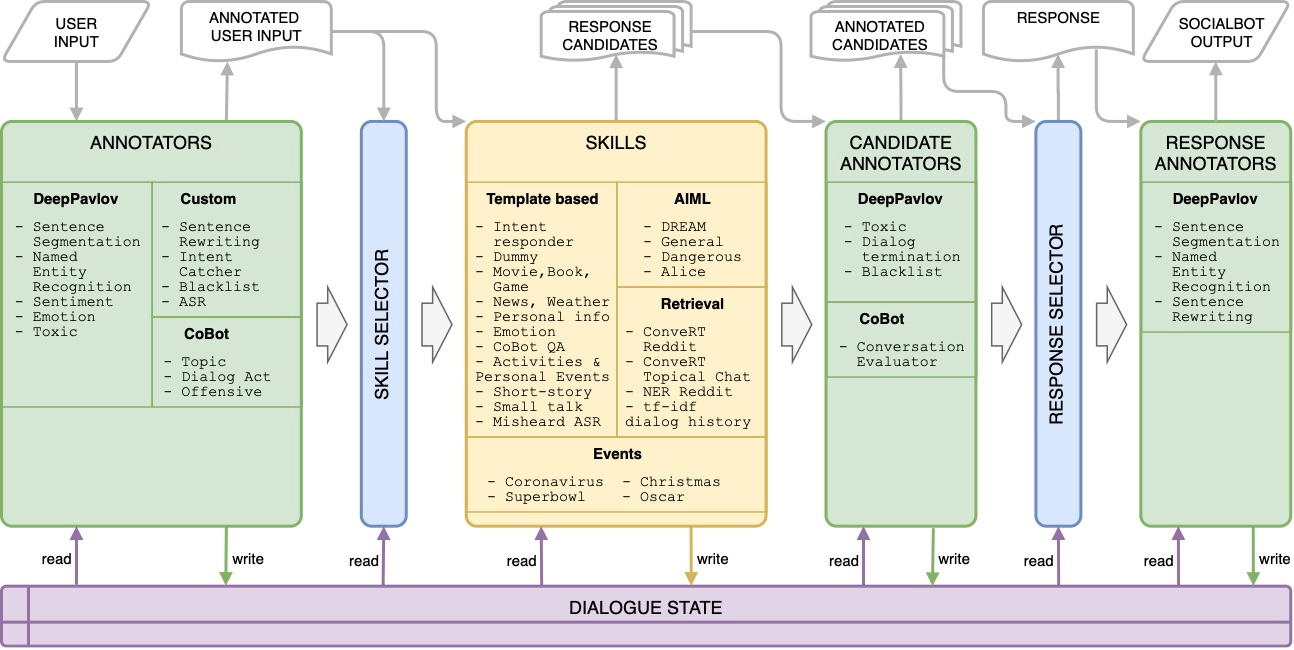
\includegraphics[width=\textwidth]{images/Alexa1_.png}
  }
  \caption{Архитектура диалоговой платформы {DREAM} в конкурсе «Alexa Prize Challenge 3»}\label{fig:Alexa1}
\end{figure}

\begin{figure}[ht]
  \centerfloat{
    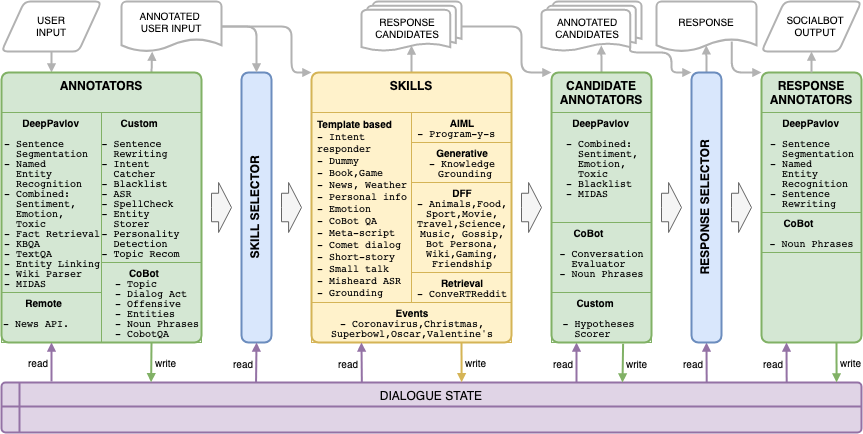
\includegraphics[width=\textwidth]{images/Alexa2_.png}
  }
  \caption{Архитектура диалоговой платформы {DREAM} в конкурсе «Alexa Prize Challenge 4»}\label{fig:Alexa2}
\end{figure}

Автор диссертационной работы внес существенный вклад в разработку диалоговой платформы DREAM, разработав или существенно улучшив ряд аннотаторов и навыков этой платформы. В их число входят:
\begin{enumerate}
 \item Навыки для обсуждения книг (Book Skill), эмоций (Emotion Skill), сплетен (Gossip Skill, коронавируса (Coronavirus Skill), слухов (Gossip Skill), для обоснования диалога (Grounding Skill), ранжирующий навык TF-IDF (TF-IDF Retrieval), а также генеративный навык, не тестировавшийся на пользователях.
 \item Аннотаторы для классификации эмоций (Emotion Classification), интентов (Intent Catcher), момента остановки диалога (Stop Detect).
\end{enumerate}

Эти аннотаторы и навыки также описаны в данной главе. 

При этом особый интерес в рамках конкурса представляла замена облачных сервисов от Amazon для тематической классификации и классификации интентов (CoBot Topics, CoBot DialogAct), а также аннотаторов для классификации эмоций, токсичности и тональности (Emotion Classification, Toxicity Classification и Sentiment classification) из Рисунка~\ref{fig:Alexa1} на аннотатор для многозадачной классификации (Combined Classification) из Рисунка~\ref{fig:Alexa2}. Этот аннотатор также является личным вкладом автора.

Необходимость данной замены была оправдана высокими издержками на эксплуатацию аннотаторов для классификации эмоций, токсичности и тональности -- каждый месяц расходовалось «кредитов» вычислительных мощностей на сумму до 9 тысяч долларов США. Помимо этого, облачные сервисы от Amazon (в названии которых есть слово Cobot) могли работать только во время конкурса, и даже во время конкурса из-за ограничений по частоте запросов работали не всегда.

Так как использование многозадачных моделей в диалоговой системе DREAM было продиктовано задачами этой платформы, задачи платформы DREAM пригодны для изучения прикладного применения многозадачных нейросетевых моделей. Подробнее эксперименты с многозадачной классификацией в диалоговой платформе DREAM описаны в шестой главе.

Все результаты, описанные в данной главе, представлены также в статьях автора~\cite{dream1,dream1_trudy,dream2,mtldream}.

\underline{\textbf{Шестая глава}} посвящена прикладному использованию многозадачных моделей, описанных в данной работе. Их прикладное использование рассматривалось на примере диалоговой платформы DREAM, описанной в предыдущей главе.

Первой версией многозадачных моделей были модели с одним линейным слоем. Эти модели использовались в диалоговой платформе DREAM для замены облачных классификаторов реплик и классификаторов качества диалога от Amazon. Модели обучались на предсказаниях соответствующих моделей от Amazon, которые были сделаны в течение первого из двух конкурсов Alexa Prize, в котором автор работы принимал участие. Данные конкурса были разбиты в соотношении 90/8/2 на тренировочную, валидационную и тестовую выборку. Тестирование для задач классификации тональности, эмоций и токсичности проводилось на их оригинальных наборах тестовых данных (упомянутых во второй главе), тестирование для задач Cobot Topics, Cobot DialogAct Topics и Cobot DialogAct Intents -- на тестовой подвыборке предсказаний соответствующих моделей от Amazon.

Заметим, что разметка для всех используемых примеров была параллельной, т.к все классификаторы от Amazon отрабатывали для каждой из реплик. Эти модели поддерживали задачи классификации токсичности, тональности и эмоций, а также замену классификаторов Cobot Topics, Cobot DialogAct Topics, Cobot DialogAct Intents. Т.е использованный подход был аналогичен подходу «Жесткие независимые метки» из третьей главы, но без объединения меток. 

Результаты этой модели представлены ниже.

\begin{table}[htbp]
    \caption{Точность (взвешенный-F1) для многозадачной классификации для различных моделей. «1 в 1» означает оригинальные модели, «6 в 1» -- многозадачную модель с одним линейным слоем, обученную на аннотациях всех упомянутых в таблице классификаторов, «3 в 1 (cobot)» -- многозадачную модель с одним линейным слоем, обученную только на аннотациях классификаторов cobot topics, cobot dialogact topics и cobot dialogact intents, «3 в 1 (не cobot)» -- многозадачную модель с одним линейным слоем, обученную только на аннотациях остальных классификаторов(классификаторы эмоций, тональности и токсичности).}
    \label{mtldream:1}
    \centering
    \scalebox{0.9}{
    \begin{tabular}{|c|c|c|c|c|} 
    \hline
    \multirow{2}{*}{3адача} & \multicolumn{4}{c|}{Модели} \\
    \cline{2-5}
     & \textbf{1 в 1} & \textbf{6 в 1} & \textbf{3 в 1 (cobot)} & \textbf{3 в 1 (не cobot)}\\ 
    \hline
    cobot topics   & --- & 84~(83) & 82~(84) & --- \\
    \hline
    cobot dialogact topics  & --- & 76~(64) & 78~(66) & --- \\ 
    \hline
    cobot dialogact intents & --- & 69~(65) & 70~(67) & --- \\ 
    \hline
    Эмоции  & 92~(75) & 82~(60) & --- & 85~(67) \\
    \hline
    Тональность & 72~(68) & 60~(57) & --- & 66~(62) \\ 
    \hline
    Токсичность & 92~(60) & 92~(59) & --- & 93~(60)\\ 
    \hline
    \end{tabular}}
\end{table}

Аналогичная модель была обучена также для замены модуля от Amazon, оценивавшего качество диалога по пяти метрикам -- ответ интересный, ответ развлекает пользователя, ответ понятный, ответ ошибочный, ответ по теме. Обученный на массиве диалогов из Alexa Prize Challenge 4, линейный слой предсказывал вектор из 5 величин от 0 до 1, метрик для мониторинга считалась средним квадратичным отклонением.

Использование данной модели дало СКО (среднеквадратичное отклонение) показателей, равное 0.31, на тестовой выборке.

Второй версией, работавшей в диалоговой платформе DREAM в течение продолжительного времени, являлась модель на основе PAL-BERT -- модели, описанной в первой главе. Эта модель показала более высокое качество, чем модель с одним линейным слоем, даже если им подавались на вход одни и те же псевдоразмеченные данные Alexa Prize, как можно видеть из следующей таблицы.

\begin{table}[htbp]
\centering
\caption {Точность (взвешенный-F1) для моделей \underline{без диалоговой истории} для многозадачной модели с 1 линейным слоем и PAL-BERT на псевдоразмеченных данных из Alexa Prize Challenge 4, оценка на «чистых» тестовых данных для не-коботовских задач и на псевдоразмеченных для коботовских задач. «1 в 1» означает оригинальные модели.}
\label{mtldream:4}
\resizebox{\textwidth}{!}{%
\begin{tabular}{|c||c|c|c|c|} \hline
\multirow{2}{*}{3адача} & \multicolumn{4}{c|}{Модели} \\
\cline{2-5}
 & 7 в 1 & \begin{tabular}[c]{@{}l@{}}7 в 1\\ жесткие метки\end{tabular} & \begin{tabular}[c]{@{}l@{}}7 в 1\\ PAL-BERT \\ жесткие метки\end{tabular} & \begin{tabular}[c]{@{}l@{}}1 в 1\\ \end{tabular} \\
\hline
\hline
cobot topics & \textbf{81.9(80)} & 80.2(78.1) & 81.8(79.5) & 1(1) \\
\hline
cobot dialogact topics & 80.5(62.6) & 79.9(61.6) & \textbf{81.4(63.2)} & 1(1) \\
\hline
cobot dialogact intents & 75.2(63.5) & 74.5(62.6) & \textbf{76.7(63)} & 1(1) \\
\hline
Эмоции & 40.1(24.5) & 72(64.1) & \textbf{78.8(75.4)} & 92(75.1) \\
\hline
Тональность & 68.3(60.7) & 72.7(60.9) & \textbf{73.3(58.5)} & 72.1(68.1) \\
\hline
Токсичность & 93.2(19.4) & 93.1(18) & \textbf{93.5(18.6)} & 92.2(59.6) \\
\hline
Фактоидность & 80.5(80.6) & 81.6(81.4) & \textbf{82.9(83.1)} & 88.6(88.4) \\
\hline
\end{tabular}
}
\end{table}


Преимущество PAL-BERT над моделью с одним линейным слоем сохранилось и после добавления в обе модели обучения на псевдоразмеченных данных, не относящихся к Alexa Prize (а именно, на псевдоразмеченных обучающих данных для не-Коботовских задач). Это позволило приблизить метрики PAL-BERT к метрикам оригинальных моделей.

Результаты этой модели в финальной серии экспериментов с PAL-BERT представлены ниже.


\begin{table}[htbp]
\centering
\caption {Точность (взвешенный-F1) для оценки моделей в третьей серии экспериментов. Для не-Коботовских задач при оценке используются оригинальные тестовые наборы данных, для коботовских -- тестовая часть разбиения данных. «1 в 1» означает оригинальные модели, «История» означает использование диалоговой истории для Коботовских задач.}
\label{mtldream:5}
\resizebox{\textwidth}{!}{%
\begin{tabular}{|c||c|c|c|c|c|c|c|} \hline
\multirow{1}{*}{} & \multicolumn{7}{c|}{Модель} \\ 
\cline{2-8}
         &7 в 1 & 7 в 1 & PAL-BERT & PAL-BERT & PAL-BERT & PAL-BERT & 1 в 1 \\
 История & нет & есть & есть & есть  & есть & есть & есть \\ \hline
 Псевдоразметка & \multirow{2}{*}{полная} & \multirow{2}{*}{полная} & \multirow{2}{*}{нет} & \multirow{2}{*}{\begin{tabular}[c]{@{}l@{}}только \\не-Коботовские \end{tabular}} & \multirow{2}{*}{полная} & \multirow{2}{*}{\begin{tabular}[c]{@{}l@{}}тональность и \\фактоидность\end{tabular}} & \multirow{2}{*}{нет} \\ 
 \cline{1-1}
Задача & & & & & & & \\
\hline
\hline
cobot topics & \textbf{70.1(66.6)} & 56.8(53.3) & 83.3(81) & 83.1(80.8) & \textbf{86.3(84.3)} & 82.8(81) & 1(1) \\
\hline
cobot dialogact topics & 75.6(51.9) & 85.2(66.7) & \textbf{87.1(70.4)} & 86.9(70.4) & \textbf{90.6(80.4)} & 86.8(69.8) & 1(1) \\
\hline
cobot dialogact intents & 51.5(40.6) & 72.8(51.6) & \textbf{76.8(56.3)} & 76.5(56.1) & \textbf{82.8(68.5)} & 75.3(55.4) & 1(1) \\
\hline
Эмоции & 90.5(88) & 91.7(88.3) & \textbf{92.7(90.6)} & 92.4(89.3) & 92.3(89.7) & 92.6(91) & 92(75.1) \\
\hline
Тональность & 72(63.3) & 71.3(65.7) & \textbf{70.6(64.8)} & 72.7(65.9) & 71.3(64.7) & \textbf{75.4(66.4)} & 72.1(68.1) \\
\hline
Токсичность & 93.8(19.9) & 93.2(21) & \textbf{92.8(25.3)} & 93.2(29.8) & 93.2(26.9) & \textbf{93.9(25.9)} & 92.2(59.6) \\
\hline
Фактоидность & 78.9(80.9) & 79.4(81.7) & \textbf{83.4(83.1)} & 84.6(84.4) & \textbf{86.9(86.6)} & 85.4(85.3) & 88.6(88.4) \\
\hline
\end{tabular}
}
\end{table}


В дальнейшем данная модель была заменена энкодер-агностичной моделью, описанной в четвёртой главе. Это было связано в первую очередь с изменениями технических требований системы DREAM, в число которых вошла возможность быстро подставлять разные базовые модели в многозадачную архитектуру. Данные требования привели к переходу на параллельную архитектуру -- а именно, энкодер-агностичную модель.


В энкодер-агностичную модель была добавлена классификация семантических интентов MIDAS и тематическая классификация DeepPavlov Topics, также были актуализированы либо дополнительно предобработаны данные для других задач.

В Таблице~\ref{tab:mtldream:final} показано, что энкодер-агностичность модели позволила заменить обычную модель дистиллированной, дополнительно выиграв в памяти.

\begin{table}[htbp]
\centering
\caption {Точность/взвешенный-F1) для оценки моделей в экспериментах с энкодер-агностичными моделями. Для не-Коботовских задач при оценке используются оригинальные тестовые наборы данных, для коботовских -- тестовая часть разбиения данных. Как distilbert обозначается модель \textit{distilbert-base-uncased}, как bert модель \textit{bert-base-uncased}. «С историей» означает использование диалоговой истории только в задаче MIDAS, «Без истории» означает, что диалоговая история не использовалась ни в одной задаче. «Размер» означает размер обучающей выборки. Режим S означает, что обучались однозадачные модели, M означает, что обучалась многозадачная модель. }
\label{tab:mtldream:final}% label всегда желательно идти после caption
\resizebox{\textwidth}{!}{
\begin{tabular}{|c|c||c|c|c||c|c|} \hline
Задача & Размер &\begin{tabular}[c]{@{}l@{}}distilbert, S\\с историей\end{tabular} & \begin{tabular}[c]{@{}l@{}}distilbert, M\\с историей\end{tabular}  & \begin{tabular}[c]{@{}l@{}}distilbert, M\\без истории\end{tabular} & \begin{tabular}[c]{@{}l@{}}bert, S\\с историей\end{tabular} & \begin{tabular}[c]{@{}l@{}}bert, M\\с историей\end{tabular}\\ \hline \hline
Эмоции              & 39.5k & \textbf{70.47/70.30} & 68.18/67.86 & 67.59/67.32         & \textbf{71.48/71.16} & 67.27/67.23 \\ \hline
Токсичность            & 162k & \textbf{94.53/93.64} & 93.84/93.5  & 93.86/93.41         & \textbf{94.54/93.15} & 93.94/93.4 \\ \hline
Тональность            & 94k  & \textbf{74.75/74.63} & 72.55/72.21 & 72.22/71.9          & \textbf{75.95/75.88} & 75.65/75.62 \\ \hline
Интенты MIDAS          & 7.1k & \textbf{80.53/79.81} & 72.73/71.56~ & 73.69/73.26 & \textbf{82.3/82.03}  & 77.01/76.38 \\ \hline
Фактоидность            & 3.6k & \textbf{81.69/81.66} & 81.02/81.07 & 80.0/79.86 & \textbf{84.41/84.44} & 80.34/80.09 \\ \hline
DeepPavlov Topics & 1.8M & \textbf{87.48/87.43} & 86.98/86.9  & 87.01/87.05         & \textbf{88.09/88.1}  & 87.43/87.47 \\ \hline
cobot topics                   & 216k & \textbf{79.88/79.9}  & 77.31/77.36 & 77.45/77.35         & \textbf{80.68/80.67} & 78.21/78.22 \\ \hline
\begin{tabular}[c]{@{}l@{}}cobot dialogact\\ topics \end{tabular}            & 127k & 76.81/76.71 & \textbf{76.92/76.79} & 76.8/76.7          & \textbf{77.02/76.97} & 76.86/76.74 \\ \hline
\begin{tabular}[c]{@{}l@{}}cobot dialogact \\intents \end{tabular}           & 318k & \textbf{77.07/77.7}  & 76.83/76.76 & 76.65/76.57         & \textbf{77.28/77.72} & 76.96/76.89 \\ \hline
Средее для 9 задач                   & 2.76M & \textbf{80.36/80.20}    & 78.48/78.22 & 78.36/78.15         & \textbf{81.31/81.12}  & 79.3/79.11 \\ \hline
\begin{tabular}[c]{@{}l@{}} Видеопамяти \\ использовано, Мб    \end{tabular}            &    & 2418*9=21762 & \textbf{2420}     & \textbf{2420}             & 3499*9=31491 & \textbf{3501}    \\ \hline
\end{tabular}
}
\end{table}

В рамках данной диссертационной работы было также проведено сравнение рассмотренной многозадачной энкодер-инвариатнтной модели с многозадачной моделью с одним линейным слоем, рассмотренной ранее. Сравнение производилось для базовой модели \textit{distilbert-base-cased} с теми же гиперпараметрами для экспериментов, что и эксперименты с этой моделью в Таблице~\ref{tab:mtldream:final}. История использовалась только в наборе данных MIDAS, как и для большинства экспериментов из этой таблицы.
В частности, энкодер-агностичная модель сравнивалась с моделью с одним линейным слоем, для которой применялись следующие способы псевдоразметки данных из Главы~2: независимые метки, мягкие независимые метки и дополненные независимые метки.
Сравнение всех этих способов приведено ниже, в Таблице~\ref{tab:mtldream:final2}.
\begin{table}[htbp]
\centering
\caption {Точность/взвешенный-F1) для оценки моделей в экспериментах с многозадачными моделями.  «Новая» означает энкодер-агностичную модель, описанную в Главе~3, «Старая» - модель с одним линейным слоем. Все модели основаны на \textit{distilbert-base-uncased}, с использованием истории только в наборе данных MIDAS. Для не-Коботовских задач при оценке используются оригинальные тестовые наборы данных, для коботовских -- тестовая часть разбиения данных. «Размер» означает размер обучающей выборки.}
\label{tab:mtldream:final2}% label всегда желательно идти после caption
\resizebox{\textwidth}{!}{
\begin{tabular}{|c||c|c|c|c|} \hline
\multirow{4}{*}{Задача}  &Новая & Старая & Старая & Старая \\
 & &             & мягкие & дополненные \\
 & & независимые & независимые & независимые \\
 & & метки & метки & метки \\ \hline \hline
Эмоции               & 68.18/67.86 & 66.2/65.96 & 57.57/50.04 & \textbf{70.14/69.98} \\ \hline
Токсичность              & 93.84/93.5  & 93.74/93.23 & 93.79/92.71 & \textbf{94.54/93.6} \\ \hline
Тональность               & 72.55/72.21 & 71.47/71.24 & 70.81/70.52 & \textbf{74.59/74.4} \\ \hline
Интенты MIDAS            & 72.73/71.56 & \textbf{74.55}/73.66 & 30.54/14.75 & 74.37/\textbf{73.86} \\ \hline
Фактоидность           & 81.02/81.07 & 79.6/79.62 & 69.02/67.17 & \textbf{81.61/81.57} \\ \hline
DeepPavlov Topics  & \textbf{86.98/86.9}  & 86.39/86.34 & 86.66/86.61 & 86.93/86.87 \\ \hline
cobot topics  & 77.31/77.36 & 60.03/59.5 & 34.22/28.74 & 78.6/78.53 \\ \hline
\begin{tabular}[c]{@{}l@{}}cobot dialogact\\ topics \end{tabular}              & \textbf{76.92/76.79} & 71.17/70.57 & 66.43/65.3 & 73.56/72.99 \\ \hline
\begin{tabular}[c]{@{}l@{}}cobot dialogact \\intents \end{tabular}            & {76.83/76.76} & 76.2/76.1 & 76.47/76.37 & \textbf{77.27/77.19} \\ \hline
Средее для 9 задач                  & \textbf{78.48/78.22} & 75.48/75.14 & 65.06/61.36 & \textbf{79.07/78.78} \\ \hline
\end{tabular}
}
\end{table}

Как можно видеть, способы, не предполагающие обучение модели с одним линейным слоем на предсказаниях однозадачных моделей (независимые метки и мягкие независимые метки) показывают себя хуже, чем энкодер-агностичная модель. При этом отставание способа «мягкие независимые метки» на задачах с достаточно большим числом классов (cobot topics, интенты MIDAS) может быть очень большим. Исключение составляют достаточно простые задачи, такие, как DeepPavlov Topics.

Чтобы модель с одним линейным слоем догнала по своему качеству энкодер-агностичную модель, необходимо применить способ «дополненные независимые метки», т.е использовать в обучающей выборке вероятности, предсказанные однозадачными моделями для тренировочных примеров из каждой задачи. Такой способ предполагает многократное увеличение времени на тренировку модели, т.к оно требует дополнительного времени на обучение каждой из моделей для псевдоразметки и получение их предсказаний, а для каждой из задач обучающих примеров после псевдоразметки становится больше, чем для энкодер-агностичной модели. 

Есть основания предполагать, что энкодер-агностичная модель и при обучении на псевдоразмеченных данных превзойдет по своему качеству модель с одним линейным слоем, но такие эксперименты в связи с большими затратами вычислительных ресурсов являются объектом будущих исследований.

По сравнению с классификаторами в версии диалоговой платформы DREAM до внедрения многозадачной энкодер-агностичной модели (т.е основанной на модели PAL-BERT) многозадачная энкодер-агностичная модель дала экономию видеопамяти в 75 процентов, экономию оперативной памяти в 57 процентов и экономию времени на классификацию в 80-85 процентов.
 
Такая большая экономия времени на классификацию в основном связана с эффектом от энкодер-агностичности. Если при использовании PAL-BERT для каждой задачи было необходимо получать предсказания многозадачной модели «с нуля», даже если они принимают одну и ту же фразу на вход, то при использовании многозадачной энкодер-агностичной модели появилась возможность один раз получить выход базового трансформера для этой фразы и дальше для всех других задачах, принимающих ее на вход, работать с этим выходом только линейными слоями, которые на порядки быстрее.

При этом, по сравнению с многозадачной моделью с одним линейным слоем, многозадачная энкодер-агностичная модель имеет ряд качественных преимуществ. Так, она не требует параллельной псевдоразметки под все задачи, что упрощает обучение модели. Проведение параллельной псевдоразметки может вносить нежелательные искажения в обучающую выборку, как показал опыт применения обученных на псевдоразмеченных данных моделей в диалоговой платформе DREAM. Помимо этого, многозадачная энкодер-агностичная модель может поддерживать не только многометочную, но и однометочную классификацию, а также ряд других задач, включающий в себя распознавание именованных сущностей или выбор между несколькими вариантами ответа.

Данные преимущества носили при выборе между этими двумя архитектурами многозадачных моделей решающий характер, несмотря на их сопоставимые показатели по расходу вычислительных ресурсов.

Энкодер-агностичная модель, помимо диалоговой платформы DREAM, была также внедрена в библиотеку DeepPavlov(версия 1.1).

%Можно сослаться на свои работы в автореферате. Для этого в файле
%\verb!Synopsis/setup.tex! необходимо присвоить положительное значение
%счётчику \verb!\setcounter{usefootcite}{1}!. В таком случае ссылки на
%работы других авторов будут подстрочными.
%Изложенные в третьей главе результаты опубликованы в~\cite{vakbib1, vakbib2}.
%Использование подстрочных ссылок внутри таблиц может вызывать проблемы.

В \underline{\textbf{заключении}} приведены основные результаты работы, которые заключаются в следующем:
%% Согласно ГОСТ Р 7.0.11-2011:
%% 5.3.3 В заключении диссертации излагают итоги выполненного исследования, рекомендации, перспективы дальнейшей разработки темы.
%% 9.2.3 В заключении автореферата диссертации излагают итоги данного исследования, рекомендации и перспективы дальнейшей разработки темы.
%ПРОСТО СКОПИРОВАЛ ПОЛОЖЕНИЯ ВЫНОСИМЫЕ ДЛЯ ЗАЩИТЫ
\begin{enumerate}
  \item {Созданная при существенном вкладе автора платформа DREAM, находящаяся в открытом доступе, пригодна для изучения прикладного применения многозадачных нейросетевых моделей.}
  %\item {На примере прикладной задачи по созданию сервиса для работы с текстами texter-ocr-cv-microservice показана применимость технологий, использованных в диалоговой платформе DREAM, за пределами этой диалоговой платформы.}
  \item {Псевдоразметка данных при помощи однозадачных моделей улучшает метрики многозадачных моделей. При этом объединение классов оправдывает себя только для задач, достаточно сильно похожих друг на друга.}
  \item {Многозадачные трансформер-агностичные нейросетевые модели показывают себя не хуже ряда других, более сложных архитектур, а предложенный метод сэмплирования - не хуже ряда других методов сэмплирования. При этом многозадачные трансформер-агностичные модели по данным проведенных экспериментов дают среднюю просадку не более 1 процента по сравнению с однозадачными моделями. При достаточной степени похожести задач друг на друга модели за счет таких задач в среднем даже превосходят однозадачные модели.}
  \item {Для достаточно малых данных многозадачные трансформер-агностичных модели начинают превосходить по своей средней точности однозадачные, в особенности - за счет задач с наименьшим объемом данных.}
  \item {Если в основе многозадачной трансформер-агностичной модели лежит многоязычный BERT, то добавление английских данных к русским при соответствующей номенклатуре классов позволяет улучшить метрики на 1-5\%. Чем меньше изначально русскоязычных данных, тем улучшение сильнее. Этот же вывод справедлив и для однозадачных моделей.}
  \item {Русскоязычные модели, обученные на 6 классах из русскоязычного набора тематических данных YAQTopics, показывают точность около 85\% на наборе данных MASSIVE. Это оправдывает использование набора данных YAQTopics для решения задачи русскоязычной тематической классификации и фундаментальных задач исследования переноса знаний.}
  \item {Для многоязычных нейросетевых моделей качество переноса знаний на разные языки на тематических данных сильно коррелирует с размером предобучающей выборки для каждого языка, но при этом не коррелирует с генеалогической близостью этого языка к языку дообучения.}
  \item {Рассмотренные многозадачные нейросетевые архитектуры пригодны для практического применения в диалоговых платформах и в рамках open-source библиотек. При этом предложенные автором трансформер-агностичные нейросетевые модели выигрывают у моделей типа PAL-BERT за счет трансформер-агностичности, а у моделей с одним линейным слоем - за счёт большей гибкости, отсутствия необходимости в псевдоразметке и как следствие - меньшей склонности к переобучению.}
\end{enumerate}


\ifdefmacro{\microtypesetup}{\microtypesetup{protrusion=false}}{} % не рекомендуется применять пакет микротипографики к автоматически генерируемому списку литературы
\urlstyle{rm}                               % ссылки URL обычным шрифтом
\ifnumequal{\value{bibliosel}}{0}{% Встроенная реализация с загрузкой файла через движок bibtex8
  \renewcommand{\bibname}{\large \bibtitleauthor}
  \nocite{*}
  \insertbiblioauthor           % Подключаем Bib-базы
  %\insertbiblioexternal   % !!! bibtex не умеет работать с несколькими библиографиями !!!
}{% Реализация пакетом biblatex через движок biber
  % Цитирования.
  %  * Порядок перечисления определяет порядок в библиографии (только внутри подраздела, если `\insertbiblioauthorgrouped`).
  %  * Если не соблюдать порядок «как для \printbibliography», нумерация в `\insertbiblioauthor` будет кривой.
  %  * Если цитировать каждый источник отдельной командой --- найти некоторые ошибки будет проще.
  %
  %% authorvak
  \nocite{dream1_trudy}%
  %
  %% authorwos
  %
  %% authorscopus
  \nocite{pseudolabel}%
  \nocite{rutopics}
  \nocite{rumtl}
  %\nocite{enmtl}
  %
  %% authorconf
  %
  %% authorother
  \nocite{dream1}%
  \nocite{dream2}%
  \nocite{Дуплякин_Дмитрий_Ондар_Ушаков_2021}

  \ifnumgreater{\value{usefootcite}}{0}{
    \begin{refcontext}[labelprefix={}]
      \ifnum \value{bibgrouped}>0
        \insertbiblioauthorgrouped    % Вывод всех работ автора, сгруппированных по источникам
      \else
        \insertbiblioauthor      % Вывод всех работ автора
      \fi
    \end{refcontext}
  }{
  \ifnum \value{citeexternal}>0
    \begin{refcontext}[labelprefix=A]
      \ifnum \value{bibgrouped}>0
        \insertbiblioauthorgrouped    % Вывод всех работ автора, сгруппированных по источникам
      \else
        \insertbiblioauthor      % Вывод всех работ автора
      \fi
    \end{refcontext}
  \else
    \ifnum \value{bibgrouped}>0
      \insertbiblioauthorgrouped    % Вывод всех работ автора, сгруппированных по источникам
    \else
      \insertbiblioauthor      % Вывод всех работ автора
    \fi
  \fi
  %  \insertbiblioauthorimportant  % Вывод наиболее значимых работ автора (определяется в файле characteristic во второй section)
 % \begin{refcontext}[labelprefix={}]    \insertbiblioexternal            % Вывод списка литературы, на которую ссылались в тексте автореферата
 % \end{refcontext}
  }
}
\ifdefmacro{\microtypesetup}{\microtypesetup{protrusion=true}}{}
\urlstyle{tt}                               % возвращаем установки шрифта ссылок URL
